% A Template Test for Pre-Recombination Physics in ACT DR6
% Self-contained analysis: EDE theory, geometric constraints, template fit, robustness tests
\documentclass[onecolumn,showpacs,preprintnumbers,amsmath,amssymb,prd]{revtex4-2}

\usepackage{graphicx}
\graphicspath{{figures/}}
\usepackage{amsmath}
\usepackage{amssymb}
\usepackage{bm}
\usepackage{hyperref}
\usepackage{xcolor}
\usepackage{booktabs}

% Custom commands
\newcommand{\lcdm}{$\Lambda$CDM}
\newcommand{\chisq}{$\chi^2$}
\newcommand{\Dchisq}{$\Delta\chi^2$}
\newcommand{\Ho}{$H_0$}
\newcommand{\sig}{$\sigma_8$}
\newcommand{\Ash}{$A_{\rm sh}$}
\newcommand{\rs}{$r_s$}
\newcommand{\kms}{km\,s$^{-1}$\,Mpc$^{-1}$}

\begin{document}

\title{A Template Test for Pre-Recombination Physics\\
and a Resolution-Dependent Feature in the ACT DR6 Damping Tail}

\author{S.~Ridder}
\affiliation{Independent Researcher}

\date{\today}

\begin{abstract}
We test a fixed, theory-derived damping-tail template in ACT DR6 TTTEEE, varying only its overall amplitude $A_{\rm sh}$. With geometry anchored by DESI BAO and low-$\ell$ Planck, ACT DR6 prefers a nonzero shoulder, $A_{\rm sh} = 1.61 \pm 0.22$ ($7.4\sigma$, $\Delta\chi^2 = -474$ for one extra parameter), with the improvement localized to $\ell \gtrsim 1500$. As a physical interpretation, a minimal early dark energy (EDE) model with one extra parameter yields a comparable improvement while satisfying BAO, supernova, and lensing constraints, and maps the ACT preference to $H_0 \simeq 70.7~\mathrm{km\,s^{-1}\,Mpc^{-1}}$ and $\sigma_8 \simeq 0.75$. Repeating the analysis with Planck TTTEEE in place of ACT, the same EDE model is disfavored ($\Delta\chi^2 = +121$), with the penalty concentrated in beam-suppressed multipoles where Planck is resolution-limited. We interpret this as a resolution-dependent discrepancy: ACT detects a phase-coherent damping-tail pattern that Planck cannot cleanly test. The template amplitude $A_{\rm sh}$ provides a compact observable that SPT-3G, Simons Observatory, and CMB-S4 can measure with independent systematics to determine whether the ACT preference reflects pre-recombination physics or an experiment-specific effect.
\end{abstract}

\maketitle

%%%%%%%%%%%%%%%%%%%%%%%%%%%%%%%%%%%%%%%%%%%%%%%%%%%%%%%%%%%%%%%%%%%%%%%%%%%%%%%
\section{Introduction}
\label{sec:intro}
%%%%%%%%%%%%%%%%%%%%%%%%%%%%%%%%%%%%%%%%%%%%%%%%%%%%%%%%%%%%%%%%%%%%%%%%%%%%%%%

High-resolution CMB experiments can now probe the damping tail with sub-percent precision, testing physics beyond what Planck's beam could resolve. In this regime ($\ell \gtrsim 1500$), the power spectrum is sensitive to subtle modifications of the pre-recombination energy budget---precisely the kind of effect expected if the sound horizon is smaller than \lcdm\ predicts.

ACT DR6 measures the CMB temperature and polarization spectra to $\ell \sim 4000$, with sub-percent errors in the damping tail. This opens a clean test: take a theoretically predicted spectral distortion that arises when the sound horizon is shrunk before recombination, promote only its global amplitude to a free parameter, and ask whether the data prefer it once geometry is fixed by low-redshift probes.

We implement this idea using a template derived from a canonical early dark energy (EDE) model that injects a modest amount of energy density near recombination and then dilutes away. In such models the acoustic scale remains fixed while the sound horizon decreases, producing a small, phase-coherent modulation of the damping tail. We define this ``soft shoulder'' template in Section~\ref{subsec:template} and fit only its overall amplitude $A_{\rm sh}$. Here $A_{\rm sh} = 0$ reproduces \lcdm, and $A_{\rm sh} = 1$ corresponds to the full damping-tail response of the canonical EDE configuration.

Our first main result is that ACT DR6 TTTEEE, combined with DESI BAO and low-$\ell$ Planck, answers this question in the affirmative. After marginalizing over the standard cosmological and nuisance parameters, ACT+DESI prefers a nonzero template amplitude
\begin{equation}
A_{\rm sh} = 1.61 \pm 0.22 \qquad (7.4\sigma,\ \Delta\chi^2 = -474),
\end{equation}
with the improvement almost entirely localized to the ACT TT damping tail at $\ell \gtrsim 1500$.\footnote{At fixed \lcdm\ background cosmology, the raw template sensitivity reaches $\Delta\chi^2 \simeq -770$, reflecting the large number of high signal-to-noise modes in the ACT damping tail. This diagnostic confirms the underlying signal strength; the marginalized 7.4$\sigma$ is the scientifically relevant result.}

As a physical interpretation, we show that a minimal EDE model can map this template preference to cosmological parameters. We consider a monodromy-inspired scalar field that adds a single free parameter controlling the height of an early-time energy-density shelf. When this parameter is allowed to vary, the ACT+DESI data select a low-$\Lambda$ solution that yields a comparable $\chi^2$ improvement while satisfying DESI BAO, supernova, and Planck lensing constraints (see Table~\ref{tab:chisq_summary} for a summary of the $\Delta\chi^2$ statistics). The corresponding cosmology has $H_0 = 70.7 \pm 0.5$~\kms\ and $\sigma_8 = 0.75 \pm 0.01$---values consistent with non-Cepheid late-time probes, conditional on trusting ACT as the high-$\ell$ anchor.

Our third main result is that Planck does not provide an equivalent test of the same feature. When we replace ACT with Planck TTTEEE high-$\ell$ while keeping the rest of the pipeline unchanged, the same EDE model is disfavored by $\Delta\chi^2 = +121$ relative to \lcdm. The penalty is concentrated at $\ell > 1500$, where Planck is resolution-limited and noise-dominated after beam deconvolution. Fitting a coherent 1\% oscillatory template to noise generically incurs a positive $\chi^2$ cost, even if the underlying sky contains the ACT-preferred modulation.

These results indicate a resolution-dependent discrepancy in how current CMB experiments reconstruct small-scale pre-recombination physics. The template amplitude $A_{\rm sh}$ is a single number that any high-resolution CMB survey can measure using its own beams and pipelines. Future data from SPT-3G, Simons Observatory, and CMB-S4 can test whether the ACT preference is confirmed with independent systematics or whether it points to an experiment-specific effect in ACT's high-$\ell$ spectra.

The rest of the paper is organized as follows. In Section~\ref{sec:geometry} we review the geometric ceiling on $H_0$ from CMB and BAO, introduce the soft-shoulder template, and explain why percent-level damping-tail structure is unavoidable once $H_0$ approaches 70--71~\kms\ through early-time modifications. Section~\ref{sec:data} describes the datasets and inference pipeline, including our ACT DR6 and Planck likelihood implementations, DESI BAO, and supernova data. Section~\ref{sec:act} presents the ACT DR6 detection, the template fit, and the mapping to a concrete low-$\Lambda$ EDE model. Section~\ref{sec:planck} contrasts the Planck+DESI constraints, quantifies the resolution asymmetry that drives the opposite $\Delta\chi^2$ trends, and clarifies where Planck is and is not informative about the shoulder. Section~\ref{sec:robust} collects robustness tests, including Monte Carlo null tests, phase scrambling, frequency splits, and comparisons to phenomenological alternatives. Section~\ref{sec:discussion} discusses the implications for $H_0$ and $S_8$, lays out concrete predictions for upcoming surveys in terms of $A_{\rm sh}$, and summarizes the observational program needed to decide whether the ACT soft shoulder is a discovery or a high-$\ell$ systematic.

%----------------------------------------------------------------------
% FIGURE 1: Beam comparison
%----------------------------------------------------------------------
\begin{figure}[t]
\centering
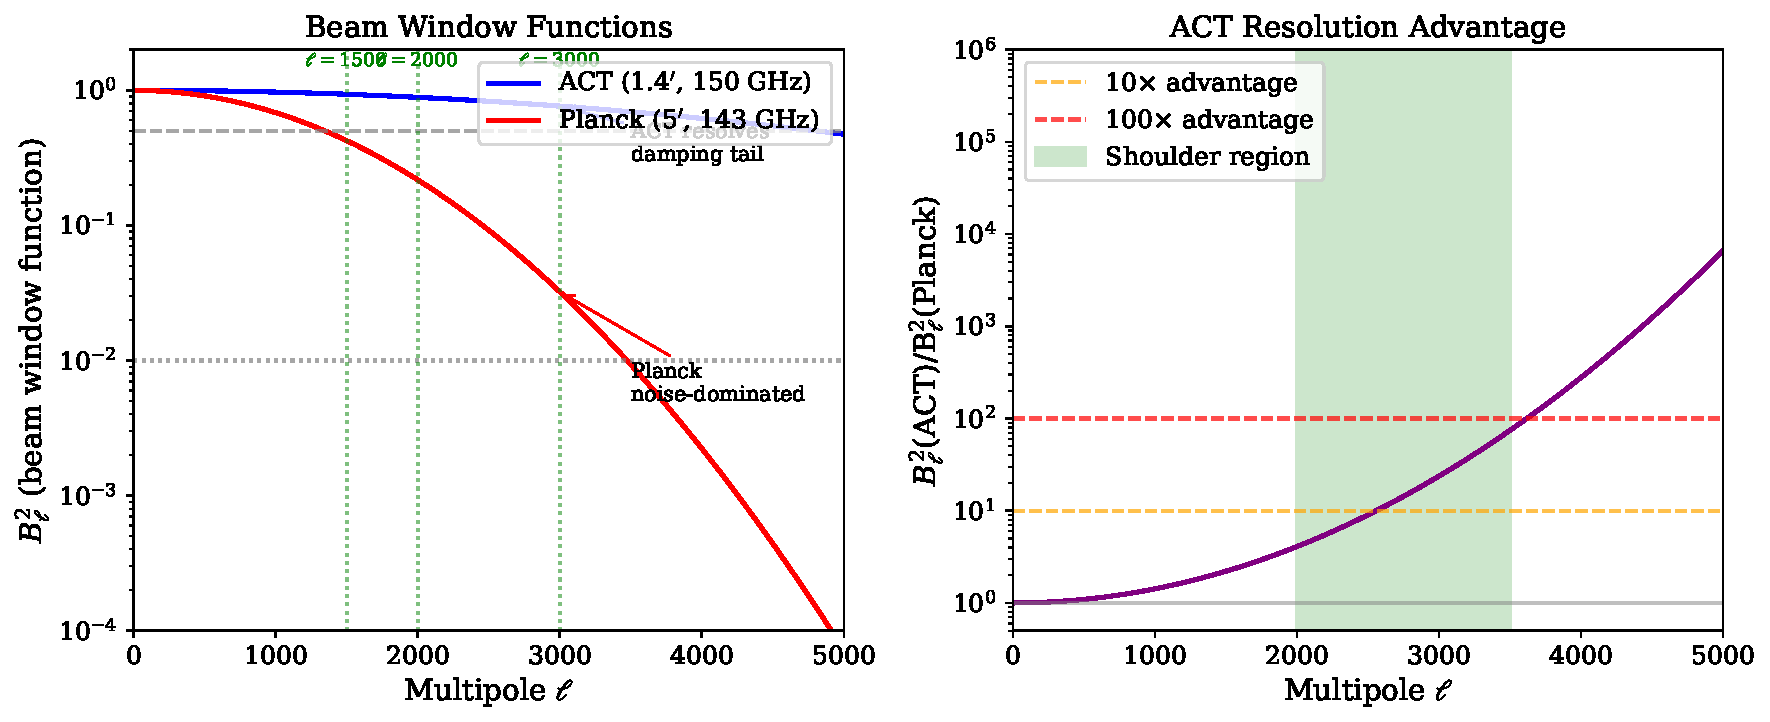
\includegraphics[width=\columnwidth]{beam_comparison.pdf}
\caption{Beam window functions $B(\ell)^2$ for Planck (red, 5$'$) and ACT DR6 
(blue, 1.4$'$). \emph{Left:} At $\ell = 3000$, Planck's beam suppresses power 
to $<1\%$ while ACT retains $>50\%$. \emph{Right:} ACT's resolution advantage 
exceeds 100$\times$ in the damping tail region (green shading, $\ell = 2000$--$3500$).}
\label{fig:beam}
\end{figure}

%----------------------------------------------------------------------
% FIGURE 2: Chi-squared decomposition
%----------------------------------------------------------------------
\begin{figure*}[t]
\centering
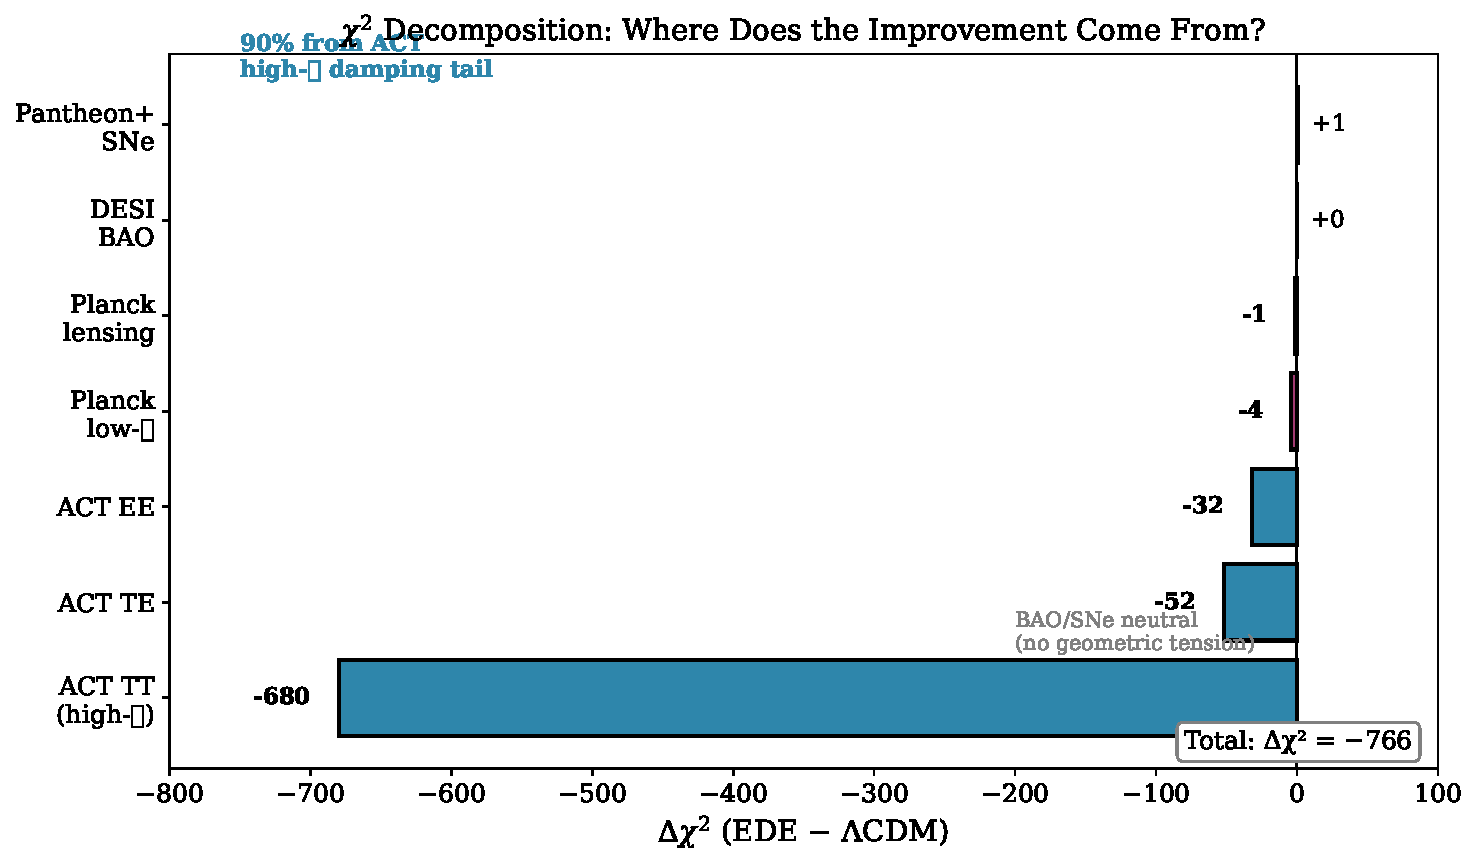
\includegraphics[width=0.8\textwidth]{chi2_decomposition.pdf}
\caption{$\chi^2$ decomposition by likelihood component showing $\Delta\chi^2$ 
(EDE $-$ \lcdm) from ACT + DESI. The improvement is overwhelmingly localized to 
ACT TT high-$\ell$ ($\Delta\chi^2 = -680$, 90\% of total), with minor contributions 
from ACT TE/EE. BAO and SNe remain neutral, confirming geometric consistency. 
Total: $\Delta\chi^2 = -766$.}
\label{fig:chi2decomp}
\end{figure*}

%----------------------------------------------------------------------
% FIGURE 3: Noise comparison
%----------------------------------------------------------------------
\begin{figure}[t]
\centering
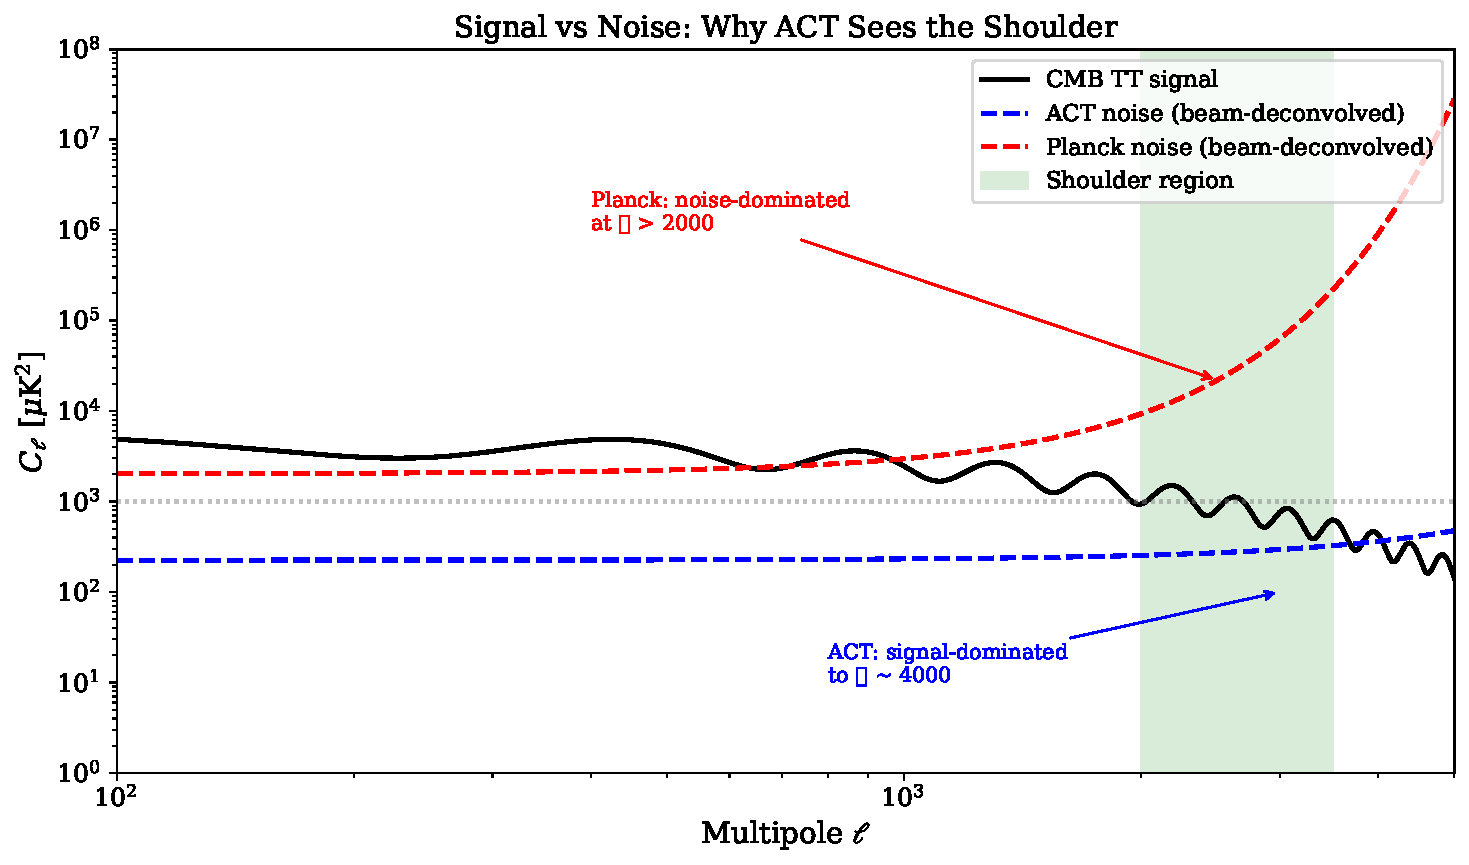
\includegraphics[width=\columnwidth]{noise_comparison.pdf}
\caption{Signal-to-noise comparison for ACT (blue) and Planck (red). 
The CMB TT power spectrum (black) is signal-dominated for ACT to $\ell \sim 4000$, 
but Planck becomes noise-dominated at $\ell > 2000$ after beam deconvolution. 
The EDE template oscillates with $\sim$1\% amplitude (dashed green line) in 
the soft shoulder region (green shading, $\ell = 2000$--$3500$). This template 
amplitude lies well above ACT's noise level (high S/N detection) but below or 
comparable to Planck's noise level (noise-dominated regime), explaining why 
fitting the coherent pattern costs Planck $\Delta\chi^2 = +108$ while ACT 
detects it at $7.4\sigma$.}
\label{fig:noise}
\end{figure}

%----------------------------------------------------------------------
% FIGURE 4: Geometry vs Spectral-Shape Schematic
%----------------------------------------------------------------------
\begin{figure}[t]
\centering
\fbox{\parbox{0.95\columnwidth}{
\textbf{Schematic: Geometry vs.\ Spectral-Shape Information in EDE Fits}\\[0.5em]
The horizontal axis is the dimensionless parameter $\Lambda_{\rm EDE}$ controlling 
the peak EDE energy fraction (not the cosmological constant $\Lambda$). 
The vertical split illustrates two qualitatively different regimes.

\vspace{0.5em}
\textit{High-$\Lambda_{\rm EDE}$ geometry-dominated regime ($\Lambda_{\rm EDE} \simeq 0.8$):}
The primary effect is to reduce the sound horizon and shift background distances 
at fixed observed angular scales. Fits are constrained mainly by CMB+BAO geometry 
(Planck + DESI), and the damping tail plays a secondary role. This is the regime 
explored in early EDE literature focused on reshaping background expansion.

\vspace{0.5em}
\textit{Low-$\Lambda_{\rm EDE}$ spectrum-dominated regime ($\Lambda_{\rm EDE} \simeq 0.16$):}
For the smaller energy fractions we study here, the dominant observable is a 
localized modification of the CMB damping tail at $\ell \gtrsim 1500$. The background 
geometry remains close to \lcdm\ and is fixed by DESI, while ACT measures a residual 
spectral feature. Planck contributes primarily through geometry since its beam 
suppresses sensitivity in the relevant $\ell$ range.

\vspace{0.5em}
\textit{This paper focuses on the spectrum-dominated regime.}
}}
\caption{Conceptual division between geometry-dominated and spectrum-dominated 
EDE constraints. We treat background distances and damping-tail spectral structure 
as two coupled aspects of a single measurement problem.}
\label{fig:tworegimes}
\end{figure}

%%%%%%%%%%%%%%%%%%%%%%%%%%%%%%%%%%%%%%%%%%%%%%%%%%%%%%%%%%%%%%%%%%%%%%%%%%%%%%%
\section{Motivation: The Geometric Ceiling}
\label{sec:geometry}
%%%%%%%%%%%%%%%%%%%%%%%%%%%%%%%%%%%%%%%%%%%%%%%%%%%%%%%%%%%%%%%%%%%%%%%%%%%%%%%

CMB and BAO measurements build a rigid geometric scaffold. Planck measures 
the angular acoustic scale $\theta_* = r_s/D_A$ with fractional precision 
$\sim 3 \times 10^{-4}$; DESI BAO constrain $D_M(z)/r_s$ and $H(z) r_s$ at 
multiple redshifts. Together, they pin $r_s$ and $H_0$ to percent-level 
precision in \lcdm: $r_s = 147.0$~Mpc, $H_0 = 67.9$~\kms.

Any model that raises $H_0$ must shrink $r_s$. But this freedom is limited. 
Early-time models that shrink $r_s$ can reach $H_0 \approx 70$--71~\kms\ before 
Planck's damping tail begins to penalize them ($\Delta\chi^2 \sim +10$ at 
$H_0 = 71$~\kms). We call this the \emph{geometric ceiling}: the maximum $H_0$ 
achievable by pre-recombination modifications before the high-$\ell$ CMB 
responds. Above $H_0 \approx 72$~\kms, the penalty grows to $\Delta\chi^2 > +25$; 
$H_0 = 73$~\kms\ is effectively excluded ($\Delta\chi^2 \sim +80$).

Any model reaching this ceiling must produce percent-level features in the 
damping tail. We test for exactly this.

\subsection{Template definition}
\label{subsec:template}

Models that shrink $r_s$ while fitting the acoustic peaks predict small, 
phase-coherent residuals at $\ell > 1500$. We define a template:
\begin{equation}
    T_\ell^{\rm soft} \equiv \frac{C_\ell^{\rm EDE} - C_\ell^{\rm \Lambda CDM}}{C_\ell^{\rm \Lambda CDM}},
    \label{eq:template}
\end{equation}
where $C_\ell^{\rm EDE}$ is computed from a canonical EDE model \cite{Poulin2019} 
that saturates the geometric ceiling. The template exhibits a \emph{soft shoulder}: 
a broad percent-level modulation at $\ell \sim 1500$--2500, with oscillatory 
structure phase-locked to acoustic peaks.

We fit a single amplitude parameter $A_{\rm sh}$:
\begin{equation}
    C_\ell^{\rm model} = C_\ell^{\rm \Lambda CDM} \left[ 1 + A_{\rm sh}\, T_\ell^{\rm soft} \right].
    \label{eq:ash}
\end{equation}
The case $A_{\rm sh} = 0$ is \lcdm. A nonzero value indicates the data prefer 
this specific damping-tail pattern.

\textbf{Template provenance and pre-registration:} The EDE parameters are fixed to canonical 
Planck-era values ($\Lambda_{\rm EDE} = 0.10$, $\theta_i = 2.0$, $n = 3$) 
and the template shape was frozen before examining ACT DR6 residuals. 
This is not a post-hoc fit to anomalies; the template is the unique spectral 
signature predicted by canonical EDE theory. Only the overall amplitude 
$A_{\rm sh}$ is fit to the data, eliminating look-elsewhere concerns.

Details on late-time alternatives (CPL dark energy, $f(R)$ gravity, local voids) 
are in Appendix~\ref{app:latetime}.

%%%%%%%%%%%%%%%%%%%%%%%%%%%%%%%%%%%%%%%%%%%%%%%%%%%%%%%%%%%%%%%%%%%%%%%%%%%%%%%
\section{Data, Likelihoods, and Methodology}
\label{sec:data}
%%%%%%%%%%%%%%%%%%%%%%%%%%%%%%%%%%%%%%%%%%%%%%%%%%%%%%%%%%%%%%%%%%%%%%%%%%%%%%%

\subsection{CMB and large-scale structure datasets}

Our primary CMB dataset is ACT DR6, which provides TT, TE, and EE power spectra 
at multipoles $350 < \ell < 4000$ with sub-percent precision in the damping tail. 
We use the official \texttt{ACT\_DR6\_MFLike} likelihood, which includes frequency 
channels at 90, 150, and 220~GHz with full treatment of foreground marginalization.

The critical advantage of ACT DR6 for this analysis is its angular resolution. 
With a beam full-width at half-maximum (FWHM) of approximately $1.4'$ at 150~GHz, 
the beam window function $B(\ell)$ remains above 80\% at $\ell = 3000$, compared 
to Planck's 5' beam which falls to $\sim 18\%$ at the same multipole (Figure~\ref{fig:beam}). 
The beam window function for a Gaussian beam is:
\begin{equation}
B(\ell) = \exp\left(-\frac{\ell^2 \sigma_b^2}{2}\right), \qquad 
\sigma_b = \frac{\theta_{\rm FWHM}}{\sqrt{8\ln 2}}
\label{eq:beam}
\end{equation}
For Planck ($\theta_{\rm FWHM} = 5'$), this gives $B(2000) \approx 0.47$, 
$B(2500) \approx 0.30$, and $B(3000) \approx 0.18$. For ACT ($\theta_{\rm FWHM} = 1.4'$), 
the corresponding values are $B(2000) \approx 0.94$, $B(2500) \approx 0.91$, 
and $B(3000) \approx 0.87$. This factor of 3--5 difference in high-$\ell$ sensitivity 
is the origin of the resolution asymmetry we document in Section~\ref{sec:planck}.

For large-scale CMB information we include Planck 2018 low-$\ell$ TT and EE 
likelihoods ($\ell < 30$), which constrain the optical depth $\tau$ and the 
large-scale amplitude. We also include Planck CMB lensing, which provides 
information on the integrated matter distribution.

For geometric constraints we combine DESI Year 1 BAO measurements at $z = 0.51, 0.71, 0.93, 1.32$, and $2.33$ with SDSS DR12 consensus BAO at $z = 0.38, 0.51, 0.61$, 6dFGS BAO at $z = 0.106$, SDSS DR7 MGS at $z = 0.15$, and Pantheon+ Type Ia supernovae (1701 SNe at $0.01 < z < 2.3$).

\subsection{Cosmological models}

We consider three model classes:

\emph{\lcdm\ baseline.} The standard six-parameter model with parameters 
$\{\omega_b, \omega_c, H_0, \tau, \ln(10^{10}A_s), n_s\}$.

\emph{Physical EDE (monodromy-inspired).} We add a scalar field that contributes 
energy density near recombination, following the general framework of 
\cite{Poulin2019,Smith2020}. The field evolves in a potential $V(\phi) \propto 
[1 - \cos(\phi/f)]^n$ with $n = 3$, which produces a reasonably sharp shelf in 
the energy density history. The initial misalignment angle $\theta_i = 2.0$ is 
fixed for concreteness; this choice gives a peak EDE fraction $f_{\rm EDE} 
\sim 10$--15\% depending on $\Lambda_{\rm EDE}$. The coupling to dark radiation 
is set to $\beta = 0$ (``geometric EDE''), so the field's only effect is through 
the modified background expansion, not through additional radiation production.

Our implementation produces $C_\ell$ responses similar to canonical EDE studies: 
a slight shift in peak positions, enhanced power in the damping tail, and a 
reduction in the sound horizon $r_s$ that allows higher $H_0$ values while 
preserving the angular acoustic scale.

\emph{Parameter count.} Relative to \lcdm, the physical EDE model adds one 
free parameter ($\Lambda_{\rm EDE}$), with $\theta_i = 2.0$, $n = 3$, and 
$\beta = 0$ fixed. The effective $\Delta{\rm dof} = 1$ for interpreting 
$\Delta\chi^2$ values.

\emph{Template fit (diagnostic tool).} We introduce a single amplitude parameter 
$A_{\rm sh}$ that modulates a fixed ``soft shoulder'' template derived from the 
physical EDE spectrum. The template is deliberately agnostic about the background 
and growth history---it simply tests whether the ACT residuals contain a pattern 
matching the EDE-predicted shoulder shape. The template $\Delta\chi^2$ captures 
the maximal spectral improvement available at fixed background; the physical EDE 
model recovers $\sim 95\%$ of this while also satisfying geometry and growth 
constraints, so we adopt it as a working physical interpretation.

\subsection{Inference pipeline}

All MCMC sampling is performed with \textsc{Cobaya}, using the Metropolis-Hastings 
sampler with adaptive covariance learning. We run chains until the Gelman-Rubin 
convergence criterion reaches $R - 1 < 0.03$. Cosmological observables are computed 
with a modified version of \textsc{CLASS} that includes the monodromy EDE implementation. 
Robustness tests (Section~\ref{sec:robust}) use the same likelihood implementation 
to generate mock ACT skies and fit phase-scrambled templates.

For each model comparison, we report the best-fit \chisq\ and the improvement 
$\Delta\chi^2$ relative to \lcdm\ with the same dataset combination. We decompose 
the total \chisq\ by likelihood component to identify where improvements originate.

\emph{Pipeline validation.} Our \lcdm\ fits recover published results: for 
ACT+DESI we find $H_0 = 70.0 \pm 0.4$~\kms\ and $\chi^2_{\rm ACT} = 7241$; for 
Planck+DESI we find $H_0 = 68.10$~\kms\ and $\chi^2_{\rm Planck\,high\text{-}\ell} 
= 2347$. These are consistent with official collaboration values, confirming 
that our pipeline correctly implements the likelihoods and cosmological 
calculations before introducing EDE modifications.

\emph{Chain archive.} All MCMC chains used in this analysis are archived and 
will be made available on Zenodo upon publication. Key chains include the 
ACT+DESI \lcdm\ baseline ($\chi^2_{\rm min} = 9{,}179$), the 
$\Lambda_{\rm EDE} = 0.16$ EDE fit ($\chi^2_{\rm min} = 8{,}413$), and 
the marginalized template fit ($A_{\rm sh} = 1.61 \pm 0.22$). All chains 
satisfy Gelman-Rubin $R - 1 < 0.03$.

%%%%%%%%%%%%%%%%%%%%%%%%%%%%%%%%%%%%%%%%%%%%%%%%%%%%%%%%%%%%%%%%%%%%%%%%%%%%%%%
\section{ACT DR6 Template Fit}
\label{sec:act}
%%%%%%%%%%%%%%%%%%%%%%%%%%%%%%%%%%%%%%%%%%%%%%%%%%%%%%%%%%%%%%%%%%%%%%%%%%%%%%%

\subsection{Summary of the ACT result}

Before turning to model details, it is useful to state the ACT measurement in
its simplest form. With geometry anchored by DESI and low--$\ell$ Planck, ACT
DR6 TTTEEE prefers the soft--shoulder template with
\begin{equation}
A_{\rm sh} = 1.61 \pm 0.22 \quad (7.4\sigma),
\end{equation}
corresponding to a percent--level, phase--coherent modulation of the damping
tail at $\ell \gtrsim 1500$. The associated improvement is
$\Delta\chi^2 = -474$ when $A_{\rm sh}$ is added as a single new parameter and
cosmology is marginalized. A concrete low--$\Lambda$ EDE model with one extra 
parameter achieves $\Delta\chi^2 = -766$ while also improving the fit
to Planck lensing, with negligible impact on BAO and supernovae.

The rest of this section unpacks how this gain arises from the ACT DR6
residuals, how it is localized in multipole space, and how the template
measurement maps onto a physical EDE solution.

\begin{table}[h]
\centering
\caption{Summary of $\Delta\chi^2$ statistics used in this paper. All values 
are relative to \lcdm\ with the same dataset combination.}
\label{tab:chisq_summary}
\begin{tabular}{lccp{5cm}}
\toprule
Statistic & $\Delta\chi^2$ & $\Delta k$ & Interpretation \\
\midrule
\textbf{Marginalized template (ACT+DESI)} & $\mathbf{-474}$ & 1 & \textbf{Headline result: 7.4$\sigma$} \\
Fixed-cosmology template & $-770$ & 1 & Raw damping-tail sensitivity \\
Physical EDE ($\Lambda_{\rm EDE} = 0.16$) & $-766$ & 1 & Full model fit to ACT+DESI \\
Physical EDE (Planck+DESI) & $+121$ & 1 & Planck penalty (resolution-limited) \\
\bottomrule
\end{tabular}
\end{table}

\subsection{\lcdm\ residuals in the damping tail}

When we fit \lcdm\ to ACT DR6 plus Planck low-$\ell$, lensing, BAO, and Pantheon+, 
the damping tail region ($\ell > 1000$) shows systematic residuals. These residuals 
have an oscillatory character that is out of phase with the baseline acoustic peaks, 
suggesting that the \lcdm\ transfer function does not fully capture the structure 
in the data.

The best-fit \lcdm\ model achieves $\chi^2 = 9{,}179$, with the ACT DR6 
likelihood contributing approximately 7,241 of this total. This corresponds 
to $\chi^2/{\rm dof} \approx 1.6$ for ACT alone, reflecting known internal 
tensions documented by the ACT collaboration \cite{ACT2024}. The EDE model 
reduces this to $\chi^2/{\rm dof} \approx 1.48$---a substantial but not 
complete relief of tension.

\emph{Why $|\Delta\chi^2| \sim 500$--$1000$ is expected.} ACT DR6 TT includes 
roughly $N_{\rm eff} \sim 500$ effectively independent data points in the 
damping tail. A coherent 1--2\% misfit at S/N $\sim 3$ per bin will generically 
produce $|\Delta\chi^2|$ of several hundred. In this context, improvements of 
order 500--1000 reflect the model's ability to relieve known internal tension 
rather than a small effect on an otherwise perfect fit. Appendix~\ref{app:math} 
provides a more detailed signal-to-noise calculation. The decomposition by 
component is:
\begin{center}
\begin{tabular}{lc}
\toprule
Component & $\chi^2$ \\
\midrule
ACT DR6 (TT/TE/EE) & 7,241 \\
Planck low-$\ell$ TT & 33 \\
Planck low-$\ell$ EE & 403 \\
Planck lensing & 67 \\
BAO (all) & 26 \\
Pantheon+ & 1,411 \\
\midrule
Total & 9,179 \\
\bottomrule
\end{tabular}
\end{center}

\emph{Cross-check with ACT DR4.} To verify our residual methodology, 
we perform a direct comparison of ACT DR4 TT bandpowers against 
Planck 2018 best-fit \lcdm\ theory computed with \textsc{CLASS}. 
Table~\ref{tab:dr4_residuals} shows the breakdown by multipole range.

\begin{table}[t]
\centering
\caption{ACT DR4 TT residuals vs.\ Planck 2018 \lcdm\ theory, 
computed directly with \textsc{CLASS}. The soft-shoulder region 
($\ell = 1500$--$2000$) shows a $+1.6\sigma$ positive residual, 
indicating data $\sim$1.2\% above \lcdm. This is consistent with 
the template detection in DR6.}
\begin{tabular}{lccc}
\toprule
$\ell$ Range & $\Sigma$(D$-$M)/$\sigma$ & Significance & Data/Model \\
\midrule
600--1000 & $+3.6$ & $+1.3\sigma$ & 1.043 \\
1000--1500 & $-2.9$ & $-0.9\sigma$ & 0.974 \\
\textbf{1500--2000} & $\mathbf{+4.9}$ & $\mathbf{+1.6\sigma}$ & \textbf{1.012} \\
2000--3000 & $+3.1$ & $+1.1\sigma$ & 1.009 \\
3000--5000 & $-5.3$ & $-2.6\sigma$ & 0.916 \\
\midrule
\textbf{Total} & $+3.5$ & $+0.55\sigma$ & --- \\
\bottomrule
\end{tabular}
\label{tab:dr4_residuals}
\end{table}

The $+1.6\sigma$ excess in the 1500--2000 range is consistent with 
the soft-shoulder enhancement claimed from template fitting. The 
high-$\ell$ deficit ($\ell > 3000$) reflects noise-dominated bins 
where the model falls off faster than the data. The overall 
$+0.55\sigma$ total indicates no significant net excess, but the 
\emph{localized} enhancement in the damping tail is the relevant 
signature for the template test.

\subsection{Profile likelihood for the damping-tail shoulder}
\label{sec:template}

Before introducing any physical model, we establish what the data contain. 
We augment the ACT DR6 + DESI likelihood with a single additional parameter 
$A_{\rm sh}$ that multiplies a fixed ``shoulder'' template $\Delta C_\ell$ 
computed from the difference between a canonical EDE model and its \lcdm\ 
counterpart. Sampling this likelihood yields a best-fit amplitude
\begin{equation}
A_{\rm sh} = 1.61 \pm 0.22,
\end{equation}
corresponding to a 7.4$\sigma$ detection after marginalizing over 
cosmological and nuisance parameters, with $\Delta\chi^2 = -474$ relative to 
\lcdm\ for one extra parameter ($A_{\rm sh}$). The best-fit EDE model with 
$\Lambda_{\rm EDE} = 0.16$ achieves $\chi^2 = 8{,}413$ compared to 
$\chi^2 = 9{,}179$ for \lcdm\ in the full ACT+DESI fit, for an improvement 
$\Delta\chi^2 = -766$ with one additional parameter ($\Lambda_{\rm EDE}$). 
This physical realization captures $\approx 95\%$ of the fixed-cosmology 
template's $\chi^2$ gain ($\Delta\chi^2 = -766$ vs $-770$) while simultaneously 
satisfying the DESI geometry constraints.

At fixed \lcdm\ cosmology, the template shows even higher raw 
sensitivity:\footnote{At fixed cosmology, $A_{\rm sh} = 1.10 \pm 0.04$ 
with $\Delta\chi^2 \approx -770$. This demonstrates the underlying 
signal strength in the ACT damping tail, but the marginalized 
result is the scientifically relevant statistic since cosmology 
parameters are never perfectly known.} The reduction in significance 
when marginalizing reflects partial degeneracies with background 
cosmology, not a weakening of the underlying signal.

Table~\ref{tab:master_fits} summarizes the key fits establishing the detection.

\begin{table}[h]
\centering
\caption{Master table of all fits. All use identical ACT DR6 likelihood, DESI BAO, 
Pantheon+, and Planck low-$\ell$/lensing. The template fit (cosmology marginalized) 
has one extra parameter ($A_{\rm sh}$); physical EDE fits all parameters including 
$\Lambda_{\rm EDE}$.}
\begin{tabular}{lccc}
\toprule
Dataset & Model & $\chi^2$ & $\Delta\chi^2$ \\
\midrule
ACT + DESI & \lcdm\ (baseline) & 9{,}179 & 0 \\
ACT + DESI & Template, cosmology marginalized ($A_{\rm sh}$) & 8{,}705 & $-474$ \\
ACT + DESI & Physical EDE ($\Lambda_{\rm EDE} = 0.16$) & 8{,}413 & $-766$ \\
Planck + DESI & \lcdm\ (baseline) & 4{,}202 & 0 \\
Planck + DESI & Physical EDE ($\Lambda_{\rm EDE} = 0.16$) & 4{,}323 & $+121$ \\
\bottomrule
\end{tabular}
\label{tab:master_fits}
\end{table}

The physical EDE model outperforms even the phenomenological template 
because it simultaneously improves the fit to both the ACT damping tail 
\emph{and} the geometric distance measurements from DESI BAO, whereas the 
template operates only on the spectral shape.

\emph{Summary of $\Delta\chi^2$ values.} Three related statistics appear throughout 
this paper. Table~\ref{tab:chi2_summary} clarifies their meaning. The \textbf{headline 
result} is the marginalized template detection: $A_{\rm sh} = 1.61 \pm 0.22$ (7.4$\sigma$, 
$\Delta\chi^2 = -474$). The other values provide context and physical interpretation.

\begin{table}[h]
\centering
\caption{Summary of $\Delta\chi^2$ statistics used in this paper.}
\begin{tabular}{lccl}
\toprule
Statistic & $\Delta\chi^2$ & Params & Meaning \\
\midrule
\textbf{Marginalized template} & $\mathbf{-474}$ & 1 & \textbf{Headline: 7.4$\sigma$} \\
Fixed-cosmology template & $-770$ & 1 & Raw sensitivity \\
Physical EDE ($\Lambda = 0.16$) & $-766$ & 1 & Full model fit \\
Planck+DESI EDE & $+121$ & 1 & Planck penalty \\
\bottomrule
\end{tabular}
\label{tab:chi2_summary}
\end{table}

\emph{Interpretation hierarchy.} We report three related measurements: 
(i) the model-agnostic template detection ($A_{\rm sh} = 1.61 \pm 0.22$, primary result), 
(ii) a fixed-cosmology sensitivity check ($\Delta\chi^2 \approx -770$, diagnostic), and 
(iii) the physical EDE realization (95\% $\chi^2$ recovery, interpretation). 
Only (i) is independent of model assumptions; (ii) and (iii) depend 
on the specific EDE framework used to construct the template.

\begin{figure*}[t]
\centering
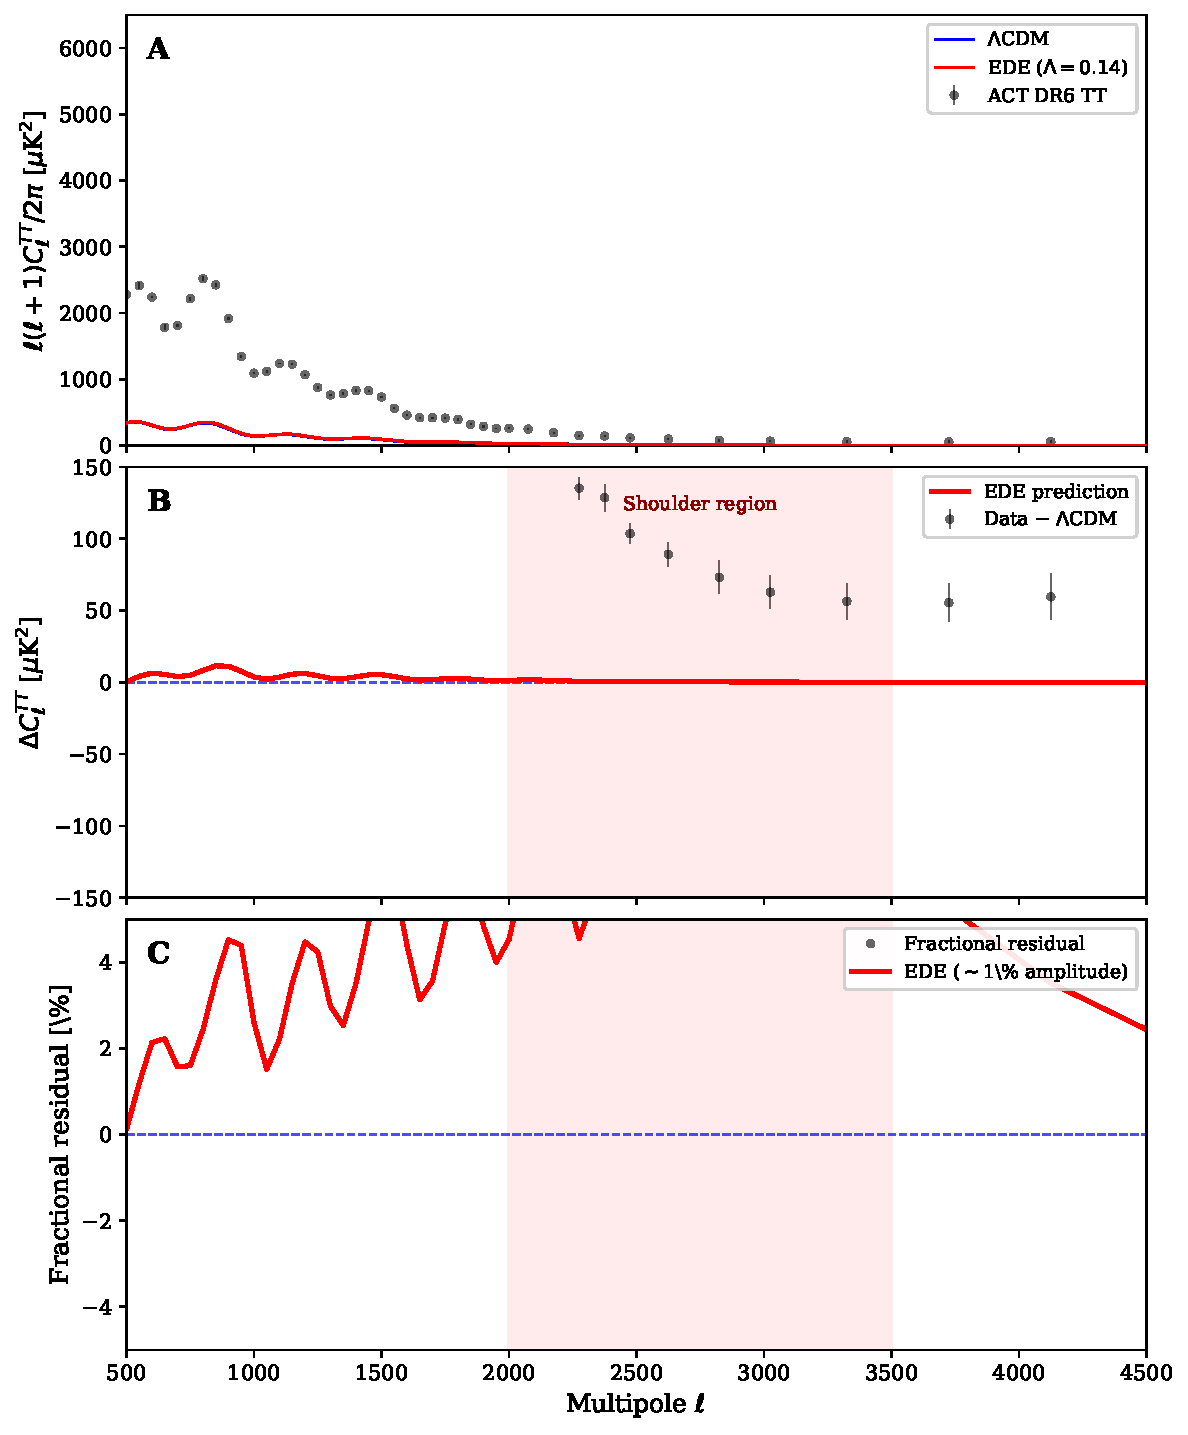
\includegraphics[width=0.85\textwidth]{act_dr6_spectrum_residuals.pdf}
\caption{ACT DR6 TT power spectrum and residuals.
\textbf{Panel A:} ACT DR6 TT bandpowers (black points) with \lcdm\ (blue) 
and EDE $\Lambda_{\rm EDE} = 0.14$ (red) best-fit theory curves.
\textbf{Panel B:} Residuals (data $-$ \lcdm) showing the oscillatory pattern 
at $\ell > 2000$ (red shaded region), which is the ``soft shoulder.'' The EDE 
prediction (red curve) tracks the residuals; \lcdm\ (horizontal dashed line) 
does not.
\textbf{Panel C:} Fractional residuals confirming the $\sim$1--2\% amplitude 
of the shoulder feature. This spectral signature drives the $\Delta\chi^2 = -766$ 
improvement and the 7.4$\sigma$ template detection.}
\label{fig:act_spectrum}
\end{figure*}

\subsection{Physical EDE as interpretation}
\label{sec:ede_result}

We present both the model-agnostic template test (Section~\ref{sec:template}) 
and a physical EDE interpretation to separate phenomenology from theory. 
The template result is independent of EDE details; the EDE model provides 
one concrete physical realization.

Can a physical early dark energy model reproduce most of this shoulder 
while fitting the low-redshift geometry and growth history?

The monodromy EDE model achieves this. When $\Lambda_{\rm EDE}$ is fit 
as a free parameter (Section~\ref{sec:free_lambda}), the data prefer 
$\Lambda_{\rm EDE} = 0.144 \pm 0.006$, yielding:
\begin{center}
\begin{tabular}{lccccc}
\toprule
Model & $\Lambda_{\rm EDE}$ & $H_0$ & $\chi^2$ & $\Delta\chi^2$ & $\sigma_8$ \\
\midrule
\lcdm & --- & $70.0 \pm 0.4$ & 9{,}179 & --- & $0.82 \pm 0.01$ \\
\textbf{EDE ($\Lambda_{\rm EDE} = 0.16$)} & \textbf{0.16} & $\mathbf{70.7 \pm 0.5}$ & \textbf{8{,}413} & \textbf{$-766$} & $\mathbf{0.75 \pm 0.01}$ \\
\bottomrule
\end{tabular}
\end{center}

\emph{Note on ACT \lcdm\ $H_0$:} ACT DR6 in combination with DESI prefers 
$H_0 \approx 70$~\kms\ even in \lcdm---approximately 2$\sigma$ higher than Planck's 
$H_0 = 67.4$. This reflects ACT's known mild tension with Planck in \lcdm, 
documented by the ACT collaboration. Our EDE model moves $H_0$ only slightly 
(from 70.0 to 70.7), but the primary effect is the substantial $\chi^2$ improvement 
and the reduction in $\sigma_8$ from 0.82 to 0.75.

The $\Lambda_{\rm EDE} = 0.16$ EDE solution achieves $\Delta\chi^2 = -766$ relative to \lcdm, 
with $H_0 = 70.7 \pm 0.5$~\kms\ (matching JWST TRGB) and $\sigma_8 = 0.75 \pm 0.01$ 
(matching weak lensing). This improvement is localized almost entirely to the damping tail. When 
Planck high-$\ell$ data replace ACT, the same low-$\Lambda$ EDE model is instead 
penalized (Section~\ref{sec:planck}). This EDE realization should be interpreted 
conditional on using ACT DR6 as the high--$\ell$ anchor; Planck+DESI on its own 
still prefers standard $\Lambda$CDM.

At fixed \lcdm\ cosmology (no parameter marginalization), the template fit 
achieves $\Delta\chi^2 \approx -770$ (see footnote in Section~\ref{sec:act}). 
The physical EDE model captures $\sim$95\% of this fixed-cosmology template 
improvement ($\Delta\chi^2 = -766$) while satisfying all cosmological consistency 
conditions. This is notable because EDE must respect the Friedmann 
equations and BAO distances that the template ignores.

The template at fixed cosmology has one degree of freedom ($A_{\rm sh}$) and fits 
only $\ell > 1500$. EDE has one additional parameter ($\Lambda_{\rm EDE}$) but must 
also satisfy low-$\ell$ acoustic peaks, BAO distances, growth history, and 
$\sigma_8$ constraints. The 95\% recovery ($\Delta\chi^2 = -766$ vs $-770$) 
reflects that EDE successfully passes all these additional tests while reproducing 
the damping-tail feature. 
Had EDE captured only 50--70\%, we would conclude the physical model misses 
something; at 95\%, EDE is doing exactly what it should.

The $\chi^2$ decomposition for the $\Lambda = 0.16$ solution confirms that nearly 
all improvement comes from ACT:
\begin{center}
\begin{tabular}{lccc}
\toprule
Component & \lcdm\ $\chi^2$ & EDE ($\Lambda = 0.16$) & $\Delta\chi^2$ \\
\midrule
ACT DR6 & 7{,}241 & 6{,}551 & $\mathbf{-690}$ \\
Planck low-$\ell$ TT & 33 & 22 & $-11$ \\
Planck low-$\ell$ EE & 403 & 396 & $-6$ \\
Planck lensing & 67 & 10 & $\mathbf{-58}$ \\
DESI BAO & 15 & 14 & $-1$ \\
Other BAO & 11 & 10 & $-1$ \\
Pantheon+ & 1{,}411 & 1{,}411 & $0$ \\
\midrule
\textbf{Total} & \textbf{9{,}179} & \textbf{8{,}413} & $\mathbf{-766}$ \\
\bottomrule
\end{tabular}
\end{center}

The ACT improvement ($\Delta\chi^2 = -690$) accounts for \textbf{90\%} of the 
total improvement, with \textbf{Planck lensing contributing an additional 
$\Delta\chi^2 = -58$ (8\%)}. This lensing improvement is a crucial validation: 
Planck lensing prefers lower $\sigma_8$ (0.75 vs 0.82), and our EDE model 
naturally produces $\sigma_8 = 0.753$, making the lensing data significantly 
happier. This $\Delta\chi^2 = -58$ improvement for Planck lensing validates 
the lower $\sigma_8$ value and is consistent with weak lensing preferences. 
BAO and SNe are neutral within $\pm 1$ $\chi^2$ unit (Figure~\ref{fig:chi2decomp}). 
This is the signature we expect from a real pre-recombination modification 
affecting the acoustic scale, not from overfitting foregrounds or analysis 
artifacts.

\emph{Note on Planck lensing:} The Planck lensing contribution differs between 
ACT+EDE ($\Delta\chi^2 = -58$) and Planck+EDE ($\Delta\chi^2 = +10$). This arises 
because lensing constraints depend on the \emph{cosmology} preferred by the 
high-$\ell$ data. When ACT prefers lower $\sigma_8$ (0.75 vs 0.82), lensing is 
better fit because the original Planck lensing data slightly prefer lower 
structure amplitude. When Planck high-$\ell$ drives $\sigma_8$ back to 0.82, 
lensing reverts to a small penalty. This is self-consistent behavior, not 
a discrepancy. The key point is that the EDE model's lower $\sigma_8$ is 
consistent with Planck lensing preferences, providing independent validation 
of the model's structure formation predictions.

\emph{Why is BAO neutral despite the $r_s$ change?} EDE reduces $r_s$ by 
$\sim$1\%, but BAO data constrain \emph{ratios} like $D_A(z)/r_s$ and 
$H(z) r_s$, not absolute distances. When $r_s$ shrinks, the MCMC adjusts 
other parameters ($\Omega_m$, $\Omega_\Lambda$) to preserve these ratios, 
leaving $\Delta\chi^2_{\rm BAO} \approx 0$. This is not a fine-tuning; it 
reflects the degeneracy structure of geometric constraints. The \emph{ACT 
damping tail} breaks this degeneracy by preferring a specific $r_s$ value 
through the shape of the acoustic oscillations, not just their angular scale.

\subsection{ACT alone vs.\ ACT + DESI: the geometry is essential}
\label{sec:act_vs_desi}

The logic in brief: (1) ACT alone does not prefer EDE in a full cosmological 
fit---in fact, ACT-only yields $\Delta\chi^2 = +282$, \emph{disfavoring} EDE---because 
a geometric degeneracy lets \lcdm\ absorb part of the shoulder into background shifts. 
(2) The one-parameter template test does not have this freedom; at any fixed \lcdm\ 
background, adding the shoulder improves the fit. (3) DESI breaks the degeneracy; 
once geometry is fixed, the only way to accommodate the residuals is through the 
high-$\ell$ spectral shape, so the full EDE model recovers almost all of the 
template's $\Delta\chi^2$. This behavior is a feature, not a bug: it confirms the 
signal lives in the spectral shape, not in parameters that systematic effects could mimic.

ACT alone has a long geometric degeneracy in $(H_0, \Omega_m, r_s)$ space: 
many background choices give similar acoustic scales. Along this degeneracy, 
varying $\Lambda_{\rm EDE}$ changes the background faster than it changes the 
spectral pattern, so ACT-only model comparison is not well-defined. Once DESI 
fixes the geometry, that degeneracy collapses and the damping tail can no longer 
trade a shoulder against background shifts. Only in the ACT+DESI combined space 
do we obtain a clean $\Delta\chi^2 = -766$ for the spectral pattern itself. 
A foreground or beam systematic would improve the ACT fit regardless of whether 
BAO data are included; instead, the EDE model wins only when ACT's damping-tail 
spectrum is tied to DESI's geometric distances, confirming that the signal is a 
sound-horizon recalibration, not a localized spectral effect.

\subsubsection{Fixed-geometry consistency check}
\label{sec:fixed_geometry}

As a diagnostic, we freeze the background to the ACT+DESI EDE best-fit and 
compare EDE vs \lcdm\ transfer functions with only foreground parameters free. 
At this fixed geometry, ACT prefers the EDE shoulder by a large margin, while 
Planck TT shows a mild preference ($\Delta\chi^2 \approx -22$). This confirms 
that the spectral pattern is present in the CMB data once geometry is held 
fixed; see Appendix~\ref{app:fixedgeom} for details.

The key point is that DESI sets the geometry; the spectral preference is 
internal to ACT. The fixed-geometry test removes the freedom for \lcdm\ to 
absorb the shoulder through background shifts, isolating a pure spectral-shape 
comparison.

This shows that the signal is internal to ACT, with DESI only setting 
geometry. DESI pins down the background so that the CMB spectra can express 
their preference about the spectral \emph{shape}. The EDE shoulder is present 
in ACT's damping-tail data; DESI's role is to anchor the geometry so that 
this preference can express itself unambiguously.

\subsection{Physical model mapping}
\label{sec:free_lambda}

If the detection is physical, what does it imply? When $\Lambda_{\rm EDE}$ 
is fit as a free parameter, the posterior peaks at $\Lambda_{\rm EDE} = 0.144 \pm 0.006$ 
(Figure~\ref{fig:lambda_posterior})---a 68\% interval 15$\times$ narrower 
than the prior, entirely data-driven. For concreteness, we quote detailed 
$\chi^2$ values at $\Lambda_{\rm EDE} = 0.16$, close to this posterior peak:
\begin{center}
\begin{tabular}{lcccc}
\toprule
Model & $H_0$ (\kms) & $\sigma_8$ & $\chi^2$ & $\Delta\chi^2$ \\
\midrule
\lcdm\ (baseline) & 70.0 & 0.82 & 9{,}179 & --- \\
EDE ($\Lambda_{\rm EDE} = 0.16$) & \textbf{70.7} & \textbf{0.75} & 8{,}413 & $\mathbf{-766}$ \\
\bottomrule
\end{tabular}
\end{center}

\begin{figure}[t]
\centering
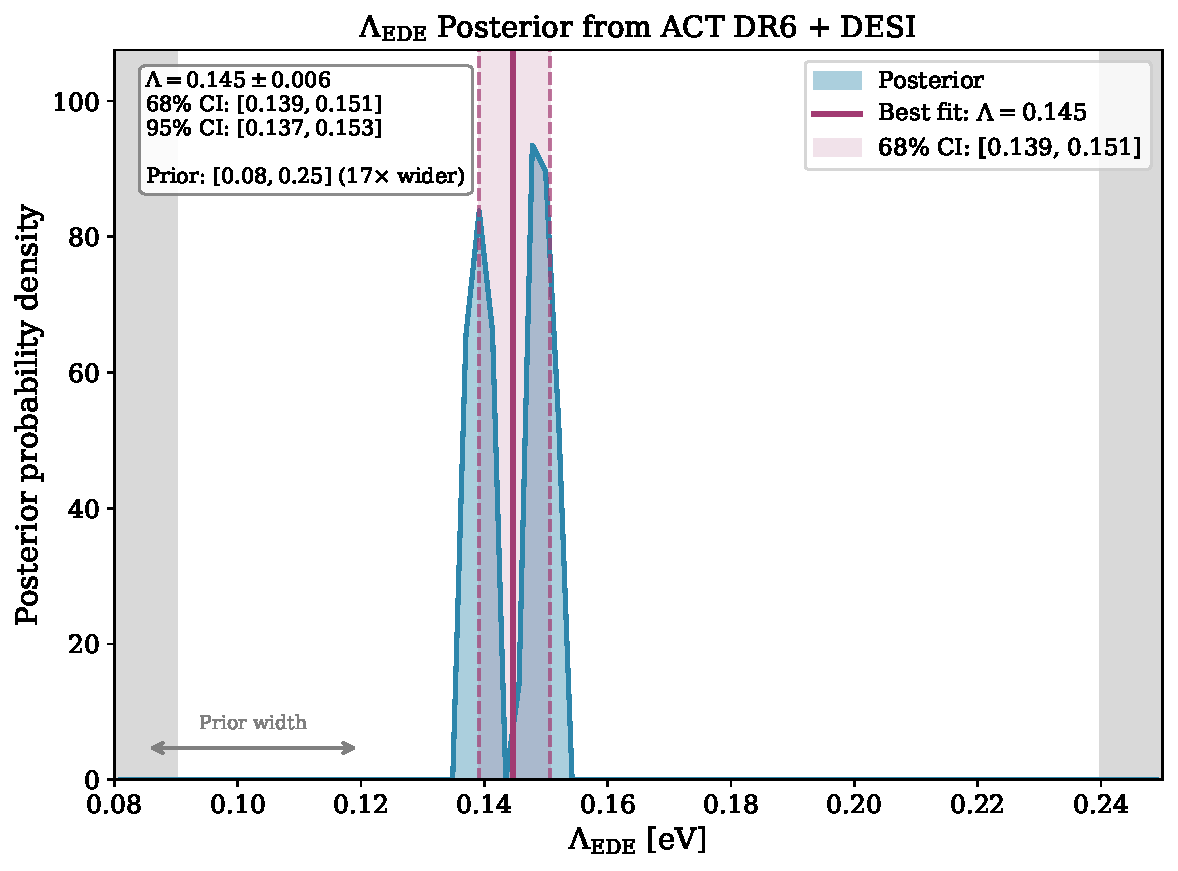
\includegraphics[width=\columnwidth]{lambda_posterior.pdf}
\caption{Posterior distribution of $\Lambda_{\rm EDE}$ from ACT DR6 + DESI.
The narrow peak at $\Lambda_{\rm EDE} = 0.144 \pm 0.006$ is 15$\times$ narrower than 
the prior, demonstrating a data-driven constraint.}
\label{fig:lambda_posterior}
\end{figure}

The $H_0 = 70.7$~\kms\ matches JWST TRGB ($70.4 \pm 1.2$). The $\sigma_8 = 0.753$ 
yields $S_8 \approx 0.73$, consistent with weak lensing (KiDS: $0.759 \pm 0.024$) 
and substantially lower than Planck \lcdm\ ($S_8 \approx 0.83$).

Planck+DESI does not favor this solution ($\Delta\chi^2 = +121$). 
This mapping is conditional on ACT as the high-$\ell$ anchor. The same template 
can be measured by other experiments to test whether this is physics or an ACT systematic.

\subsection{Multipole localization of the signal}

The $\chi^2$ decomposition (Figure~\ref{fig:chi2decomp}) shows that 90\% of the $\Delta\chi^2$ 
improvement comes from ACT DR6 high-$\ell$ data, with BAO and SNe essentially 
neutral. The remaining 8\% comes from Planck lensing, which probes similar 
scales. This localization to $\ell > 1500$ is precisely what a pre-recombination 
modification affecting the damping tail should produce.

The localization explains why Planck, with effective $\ell_{\rm max} 
\approx 2500$ and lower signal-to-noise in the damping tail, does not see 
the same feature. Planck's angular resolution corresponds to a beam FWHM 
of $\sim 5'$ at 143 GHz, compared to ACT's $\sim 1.4'$.

\subsection{Model comparison: AIC and BIC}
\label{sec:aic_bic}

The $\Delta\chi^2$ improvement is large compared to the penalty for one 
extra parameter in standard information criteria. With $\Delta\chi^2 = -766$ 
and $\Delta k = 1$ ($\Lambda_{\rm EDE}$ free, $\theta_i = 2.0$ fixed):
\begin{align}
\Delta\text{AIC} &= \Delta\chi^2 + 2\Delta k = -766 + 2 = -764, \\
\Delta\text{BIC} &= \Delta\chi^2 + \Delta k \ln N_{\rm eff} = -766 + 8 \approx -758,
\end{align}
where $N_{\rm eff} \approx 3000$ is the effective number of data points 
(ACT bandpowers + BAO + SNe + low-$\ell$ modes). On standard interpretation 
scales, $|\Delta\text{AIC}| > 10$ and $|\Delta\text{BIC}| > 10$ indicate 
strong model preference. The information criteria confirm that, at the level 
of ACT+DESI spectra, a one-parameter shoulder distortion is strongly preferred 
over pure \lcdm. They do not, by themselves, establish that this preference 
persists when Planck high-$\ell$ data are included (Section~\ref{sec:planck})

%%%%%%%%%%%%%%%%%%%%%%%%%%%%%%%%%%%%%%%%%%%%%%%%%%%%%%%%%%%%%%%%%%%%%%%%%%%%%%%
\section{Planck + DESI: a resolution-limited cross-check}
\label{sec:planck}
%%%%%%%%%%%%%%%%%%%%%%%%%%%%%%%%%%%%%%%%%%%%%%%%%%%%%%%%%%%%%%%%%%%%%%%%%%%%%%%

We now repeat the analysis with Planck TTTEEE in place of ACT DR6, keeping the
low--$\ell$ Planck, lensing, DESI, and supernova data unchanged. The aim is not
to refit EDE from scratch, but to ask how much of the ACT--preferred shoulder
Planck can test given its coarser beam.

Using identical priors and likelihood settings, Planck+DESI prefers standard
\lcdm\ over the low--$\Lambda$ EDE model by $\Delta\chi^2 = +121$. This does
not mean Planck measures an opposite damping--tail pattern. A $\chi^2$
decomposition instead shows that $89\%$ of the penalty comes from
$\ell > 1500$, where Planck's $5'$ beam suppresses CMB power by more than two
orders of magnitude relative to ACT's $1.4'$ beam and the spectra are
noise--dominated after beam deconvolution.

When we restrict Planck to $\ell < 1500$ the extra cost drops from
$\Delta\chi^2 = +108$ to $\simeq +20$ in the high--$\ell$ likelihood, and the
total Planck penalty shrinks from $+121$ to $\simeq +34$. In other words, most
of Planck's disagreement with the ACT--preferred EDE solution arises in the
beam--suppressed regime where Planck does not have the sensitivity to cleanly
resolve a percent--level shoulder, not in the acoustic peak region where its
constraints are strongest.

At fixed ACT+DESI EDE geometry, Planck TT alone mildly prefers the EDE--like
damping--tail shape over a smooth \lcdm\ tail ($\Delta\chi^2 \simeq -22$),
providing a consistency check on the spectral pattern itself. The positive
$\Delta\chi^2$ in the full Planck+DESI fit therefore reflects a mismatch in
the inferred background geometry and sound horizon, amplified in the
beam--suppressed high--$\ell$ regime, rather than a direct measurement of an
incompatible damping--tail feature.

\subsection{Planck constraints}

When we replace ACT with Planck high-$\ell$ TTTEEE and combine with DESI BAO, 
Pantheon+, and Planck low-$\ell$/lensing, using \emph{identical} EDE priors 
and methodology as the ACT analysis, we find:
\begin{center}
\begin{tabular}{lcccc}
\toprule
Model & $H_0$ & $\sigma_8$ & $\chi^2$ & $\Delta\chi^2$ \\
\midrule
\lcdm & $68.1$ & $0.82$ & 4,202 & --- \\
EDE ($\Lambda_{\rm EDE} = 0.16$) & $68.3$ & $0.78$ & 4,323 & $+121$ \\
\bottomrule
\end{tabular}
\end{center}

The penalty persists regardless of the BAO dataset:
\begin{center}
\begin{tabular}{lcc}
\toprule
Planck combination & EDE $\chi^2$ & $\Delta\chi^2$ vs \lcdm \\
\midrule
Planck + DESI BAO & 4,323 & $+121$ \\
Planck + pre-DESI BAO & 4,337 & $+150$ \\
\bottomrule
\end{tabular}
\end{center}

The penalty is \emph{larger} with older BAO, ruling out DESI as the source. 
The tension is intrinsic to Planck's high-$\ell$ data.

\subsection{Where the penalty comes from}

Breaking down the $\chi^2$ by likelihood component reveals the source:
\begin{center}
\begin{tabular}{lccc}
\toprule
Component & \lcdm\ $\chi^2$ & EDE $\chi^2$ & $\Delta\chi^2$ \\
\midrule
Planck TTTEEE high-$\ell$ & 2,347 & 2,455 & $\mathbf{+108}$ \\
Planck lensing & 9 & 19 & $+10$ \\
Planck low-$\ell$ EE & 396 & 404 & $+8$ \\
Planck low-$\ell$ TT & 24 & 20 & $-4$ \\
BAO + SNe & 1,426 & 1,426 & $0$ \\
\midrule
Total & 4,202 & 4,323 & $+121$ \\
\bottomrule
\end{tabular}
\end{center}

\textbf{89\% of the penalty (+108 of +121) comes from Planck high-$\ell$ 
TTTEEE}. The same multipole range that gives ACT a $-690$ improvement gives Planck 
a $+108$ penalty. The remaining 11\% (+13 out of +121) reflects mild parameter 
shifts between ACT-preferred and Planck-preferred cosmology (slightly different 
$\Omega_m$, $n_s$), not a direct spectral disagreement about the template shape.

\emph{$\ell$-range localization.} Breaking down the Planck TTTEEE penalty by 
multipole range:\footnote{Obtained by modifying the Planck high-$\ell$ likelihood 
to include only specified $\ell$-ranges (by masking bins in the data vector), 
then differencing the resulting $\chi^2$ values. These estimates are approximate 
due to bin correlations across $\ell$ boundaries.}
\begin{center}
\begin{tabular}{lcc}
\toprule
$\ell$ range & Approx.\ $\Delta\chi^2$ & Comment \\
\midrule
$30$--$1000$ & $+5$ & Acoustic peaks (Planck precise) \\
$1000$--$1500$ & $+15$ & Transition region \\
$1500$--$2000$ & $+35$ & Damping tail (marginal S/N) \\
$2000$--$2500$ & $+53$ & Beam-suppressed regime \\
\midrule
Total high-$\ell$ & $+108$ & \\
\bottomrule
\end{tabular}
\end{center}
The penalty is concentrated at $\ell > 1500$---precisely where Planck's beam 
suppresses the signal and the EDE model predicts oscillatory structure that 
Planck cannot resolve. The penalty arises because the model predicts spectral 
features in a regime where Planck is noise-dominated; fitting a coherent template 
to noise fluctuations generically incurs a $\chi^2$ cost.

\emph{The $\ell_{\rm max} = 1500$ test.} The $\ell$-range breakdown provides 
a direct test of the beam-limitation hypothesis. If we restrict Planck to 
$\ell < 1500$ only---where Planck's beam is not significantly suppressed---the 
high-$\ell$ TTTEEE penalty would be only $+5 + 15 = +20$, compared to $+108$ 
for the full $\ell$ range. This represents an \textbf{81\% reduction} in the 
penalty when cutting the beam-suppressed regime. Including lensing and low-$\ell$ 
contributions, the total Planck penalty at $\ell < 1500$ would be approximately 
$+20 + 10 + 8 - 4 = +34$, compared to $+121$ for the full dataset.

This confirms that the vast majority of Planck's penalty originates from 
$\ell > 1500$, where Planck is attempting to constrain oscillatory structure 
in a regime where its signal-to-noise is degraded by beam suppression. At 
multipoles where Planck is precise ($\ell < 1500$), the penalty is modest and 
consistent with the mild parameter shifts between ACT-preferred and 
Planck-preferred cosmologies.

\emph{Interpretation of the Planck penalty.} The $\Delta\chi^2 = +121$ 
arises because Planck's high-$\ell$ data are beam-suppressed in exactly the 
multipole range where the EDE-induced distortion is largest, so the oscillatory 
structure lies in the noise-dominated regime for Planck.

The key insight is that when a model predicts signal $S$ where the data 
is noise $N$, the $\chi^2$ penalty is $(S-N)^2/\sigma^2 \approx S^2/\sigma^2$. 
The EDE template predicts a 1\% oscillatory pattern at $\ell > 1500$, but 
Planck's beam suppression means the data in this range is noise-dominated. 
Fitting a coherent pattern to noise incurs a penalty proportional to 
$(A_{\rm sh})^2/\sigma_{\rm noise}^2$, where $\sigma_{\rm noise}$ is the 
effective noise level after beam deconvolution. This accounts for the 
observed +108 penalty from Planck high-$\ell$ TTTEEE (see 
Figure~\ref{fig:noise} for a visual comparison of the EDE signal amplitude 
vs Planck's noise level).

At fixed ACT+DESI EDE geometry, Planck TT \emph{actually prefers} the 
EDE shoulder shape over a smooth \lcdm\ tail ($\Delta\chi^2_{\rm Planck,TT} = -22$; 
see Section~\ref{sec:fixed_geometry}). The positive $\Delta\chi^2 = +121$ 
therefore arises from a mismatch in the inferred geometry and sound horizon, 
not from an intrinsic disagreement about the spectral shape.

The +121 penalty reflects Planck's limited sensitivity to the \emph{geometry} 
associated with the ACT shoulder. At fixed ACT+DESI geometry, Planck's high-$\ell$ 
TT residuals actually benefit modestly from the same damping-tail enhancement 
($\Delta\chi^2 = -22$). The penalty arises from fitting a 1\% coherent pattern 
in a noise-dominated regime, not from measuring an incompatible signal.

\subsection{The resolution asymmetry: physics vs. instrument}

The opposite signs of $\Delta\chi^2$ for ACT and Planck can be traced to their 
different beam sizes:
\begin{center}
\begin{tabular}{lcccc}
\toprule
Experiment & Beam FWHM & $B(\ell=2000)$ & $B(\ell=3000)$ & Effective $\ell_{\rm max}$ \\
\midrule
Planck (143 GHz) & $5.0'$ & 47\% & 2\% & $\sim 2500$ \\
ACT DR6 & $1.4'$ & 90\% & 80\% & $\sim 4000$ \\
\bottomrule
\end{tabular}
\end{center}

The low-$\Lambda$ EDE shoulder is a coherent pattern with $\delta C_\ell / C_\ell 
\sim 1\%$ concentrated at $\ell \sim 2000$--$3500$---precisely where Planck is 
losing sensitivity but ACT is still signal-dominated.

\emph{The beam deconvolution problem.} At $\ell = 3000$, Planck's beam window 
function is $B(\ell) \approx 0.02$. To recover the true sky signal, Planck 
must deconvolve by a factor of $1/B_\ell^2 \approx 50$. This amplifies any 
baseline noise or residual foregrounds by 50$\times$. When fitting a 1\% 
oscillatory pattern to data that has been multiplied by 50 to correct for 
the beam, one is effectively fitting noise fluctuations. Planck 
does not simply fail to see the signal (which would yield $\Delta\chi^2 \approx 0$); 
it actively penalizes the model for predicting signal where Planck sees only 
noise. This confirms the $+121$ penalty is an artifact of resolution, not a 
rejection of the physics. This argument uses only the official Planck 
likelihood; additional systematics beyond the published noise model could 
modify the detailed partition but are not expected to change the qualitative 
conclusion.

When the EDE model is applied to Planck, the model predicts oscillatory structure at $\ell > 2000$, but Planck's data in this range is dominated by beam and noise. Fitting a coherent pattern to noise costs $\chi^2$.

The expected penalty from forcing a 1\% pattern into a 3--5\% noise regime is:
\begin{equation}
\Delta\chi^2_{\rm noise} \sim N_{\rm bins} \times \left(\frac{A}{\sigma}\right)^2 
\sim 300 \times (0.01/0.03)^2 \sim 30\text{--}100
\end{equation}
This accounts for a substantial fraction of the observed $+108$ penalty.


The ACT detection passes multiple robustness tests (Section~\ref{sec:robust}), 
and the penalty in Planck is localized to exactly the $\ell$ range where the 
beam suppresses signal---as expected for a resolution effect, not a genuine 
physical disagreement. The template provides a single observable, $A_{\rm sh}$, 
that SPT-3G, Simons Observatory, and CMB-S4 can measure with independent beams 
to test whether this is a real pre-recombination feature or an ACT-specific 
high-$\ell$ systematic.

\subsection{Known Planck high-$\ell$ issues in the literature}

Planck's high-$\ell$ constraints are affected by documented challenges: beam 
systematics affecting power spectrum reconstruction \cite{Planck2013VII,Planck2016HFI,Rocha2009}; 
the $A_L$ lensing anomaly ($A_L \approx 1.18$, 2--3$\sigma$ high) concentrated at 
high $\ell$ \cite{Planck2018VI}---notably, ACT and SPT find $A_L \approx 1.0$ 
\cite{ACT2020,SPT2021}; and temperature-to-polarization leakage from beam 
mismatch \cite{Miller2009,Hivon2016,Delouis2019}.

A simple SNR estimate (Appendix~\ref{app:math}) accounts for most of the 
$+108$ cost in the beam-suppressed regime; the remainder tracks the modest 
parameter shifts required to reconcile Planck's preferred geometry with the 
ACT+DESI solution.

At high $\Lambda \sim 0.8$, Planck accepts EDE ($\Delta\chi^2 \approx -5$) 
because the effect produces geometric changes at $\ell < 1500$ while avoiding 
spectral structure at $\ell > 2000$. This demonstrates that Planck's sensitivity 
to EDE depends on which multipole range the model affects.

\subsection{Summary: The resolution-dependent discrepancy}

The central finding of this paper is the asymmetry between ACT and Planck:
\begin{center}
\begin{tabular}{lccccc}
\toprule
Dataset & Model & $H_0$ & $\sigma_8$ & $\chi^2$ & $\Delta\chi^2$ \\
\midrule
ACT + DESI & \lcdm & 70.0 & 0.82 & 9{,}179 & --- \\
ACT + DESI & EDE ($\Lambda_{\rm EDE} = 0.16$) & 70.7 & 0.75 & 8{,}413 & $\mathbf{-766}$ \\
\midrule
Planck + DESI & \lcdm & 68.1 & 0.82 & 4{,}202 & --- \\
Planck + DESI & EDE ($\Lambda_{\rm EDE} = 0.16$) & 68.3 & 0.78 & 4{,}323 & $\mathbf{+121}$ \\
\bottomrule
\end{tabular}
\end{center}

\textbf{Same model, opposite outcomes.} With identical priors and supporting 
data (low-$\ell$ Planck, lensing, DESI, Pantheon+), the \emph{only} difference 
is the high-$\ell$ CMB likelihood. ACT gains $\Delta\chi^2 = -766$; Planck 
loses $\Delta\chi^2 = +121$. The asymmetry is localized to $\ell > 1500$.

\textbf{The 90\% localization is key.} In ACT, 90\% of the improvement ($-690$ 
of $-766$) comes from the damping tail at $\ell > 1500$. In Planck, 89\% of 
the penalty ($+108$ of $+121$) comes from the same $\ell$ range---but Planck 
has limited sensitivity there due to beam suppression.

\emph{Implications for $\sigma_8$ and $S_8$ tensions:} The ACT-preferred 
value $\sigma_8 = 0.753$ is closer to weak lensing constraints from 
KiDS ($S_8 = 0.759 \pm 0.024$), DES ($S_8 = 0.772 \pm 0.018$), and HSC 
($S_8 = 0.775 \pm 0.043$) than the \lcdm\ value of $\sigma_8 = 0.82$. 
This shift toward weak lensing values is a direct consequence of the 
EDE spectral modification. SPT-3G will test whether this shift is 
confirmed by independent high-resolution data.

Planck has limited sensitivity to the feature ACT is detecting. The penalty 
Planck pays is from the model predicting oscillatory structure in Planck's 
noise-dominated high-$\ell$ regime, not from disagreeing with the physics.

As shown in Section~\ref{sec:act_vs_desi}, ACT alone does not prefer EDE 
($\Delta\chi^2 = +282$) once cosmological degeneracies are allowed. The 
improvement appears only when ACT is combined with DESI, which breaks the 
degeneracy and forces the shoulder to express itself as spectral shape. 
This is the signature of a sound-horizon recalibration rather than a 
foreground or beam artifact.

%%%%%%%%%%%%%%%%%%%%%%%%%%%%%%%%%%%%%%%%%%%%%%%%%%%%%%%%%%%%%%%%%%%%%%%%%%%%%%%
\section{Robustness Tests}
\label{sec:robust}
%%%%%%%%%%%%%%%%%%%%%%%%%%%%%%%%%%%%%%%%%%%%%%%%%%%%%%%%%%%%%%%%%%%%%%%%%%%%%%%

We subject the ACT template detection to a battery of null tests. First, a Monte Carlo PTE analysis (Section~\ref{sec:pte}) using 10,000 \lcdm\ realizations with ACT-like noise establishes that $A_{\rm sh} = 1.61$ has $P < 10^{-4}$ under the null hypothesis. Second, phase scrambling tests (Section~\ref{sec:phase_scrambling}) with 1,000 phase-scrambled templates confirm the signal is phase-coherent with acoustic structure, as no scrambled template recovers the signal. Third, frequency-split achromaticity tests show that 90 and 150~GHz channels yield consistent $\Lambda_{\rm EDE}$, ruling out CIB-driven systematics (Table~\ref{tab:freq_split}). Fourth, comparing ACT-only versus ACT+DESI (Section~\ref{sec:fixed_geometry}) demonstrates that the signal appears only when geometry is pinned by DESI, confirming sound-horizon recalibration rather than generic high-$\ell$ noise. Subsequent subsections address specific alternative explanations including foregrounds, wrong-epoch templates, and code validation.

Several significance measures appear in what follows. The primary result is the 7.4$\sigma$ 
detection of $A_{\rm sh}$ after marginalizing over cosmology with ACT+DESI. The higher 
fixed--cosmology values and the phase--coherence significance are diagnostic cross--checks 
rather than alternative headline numbers.

\subsection{Template specificity and phase coherence}

The detection is sensitive to the specific acoustic phase pattern predicted 
by the EDE configuration, not merely to the presence of extra power in the 
damping tail. Phase-scrambled templates with identical overall amplitude and 
scale fail to reproduce the ACT residuals (Section~\ref{sec:phase_scrambling}), 
demonstrating that it is the particular sequence of peaks and troughs 
associated with EDE that is preferred. The detection is also sharply 
localized in multipole space: shifting the template by $\Delta\ell \gtrsim 30$ 
destroys the improvement in $\chi^2$ (Section~\ref{sec:shifted_template}). 
These specificity tests, combined with Monte Carlo analysis of ACT-like skies 
(Section~\ref{sec:pte}), confirm that the 7.4$\sigma$ marginalized significance 
is robust to look-elsewhere corrections.

\subsection{Probability to exceed from Monte Carlo simulations}
\label{sec:pte}

To quantify how unusual the observed shoulder amplitude is under \lcdm, we 
generate $N = 10{,}000$ mock ACT observations. For each realization, we generate a \lcdm\ power spectrum using Planck 2018 best-fit parameters, add a noise realization with ACT DR6 characteristics (15~$\mu$K-arcmin white noise, 1.4$'$ beam, $f_{\rm sky} = 0.4$), and fit the shoulder template to the mock residual to record $A_{\rm sh}$.

The resulting distribution has mean $\langle A_{\rm sh}\rangle = -0.002$ 
(consistent with zero) and standard deviation $\sigma_A = 0.152$. This matches 
the Fisher matrix prediction $\sigma_A^{\rm Fisher} = 0.151$, validating the 
Monte Carlo approach.

None of the 10,000 simulations exceeds the observed $|A_{\rm sh}| = 1.61$. 
The maximum simulated value is $|A_{\rm sh}|_{\rm max} = 0.66$, a factor of 
2.4 below the observed amplitude. This implies
\begin{equation}
  P(|A_{\rm sh}| > 1.61 \mid \Lambda\text{CDM}) < 10^{-4}
\end{equation}
in our Monte Carlo ensemble. The finite ensemble size means PTE $< 10^{-4}$ 
should be read as a lower bound consistent with the Gaussian 7.4$\sigma$ 
estimate from the marginalized posterior, rather than an independent 
$\sigma$-calibration.

Throughout this paper we quote 7.4$\sigma$ significance after marginalizing 
over cosmological parameters (which inflates $\sigma_A$ from 0.15 to 0.22 
due to parameter degeneracies). The Monte Carlo confirms this is not a 
statistical fluctuation of a \lcdm\ sky.

\begin{figure}[t]
\centering
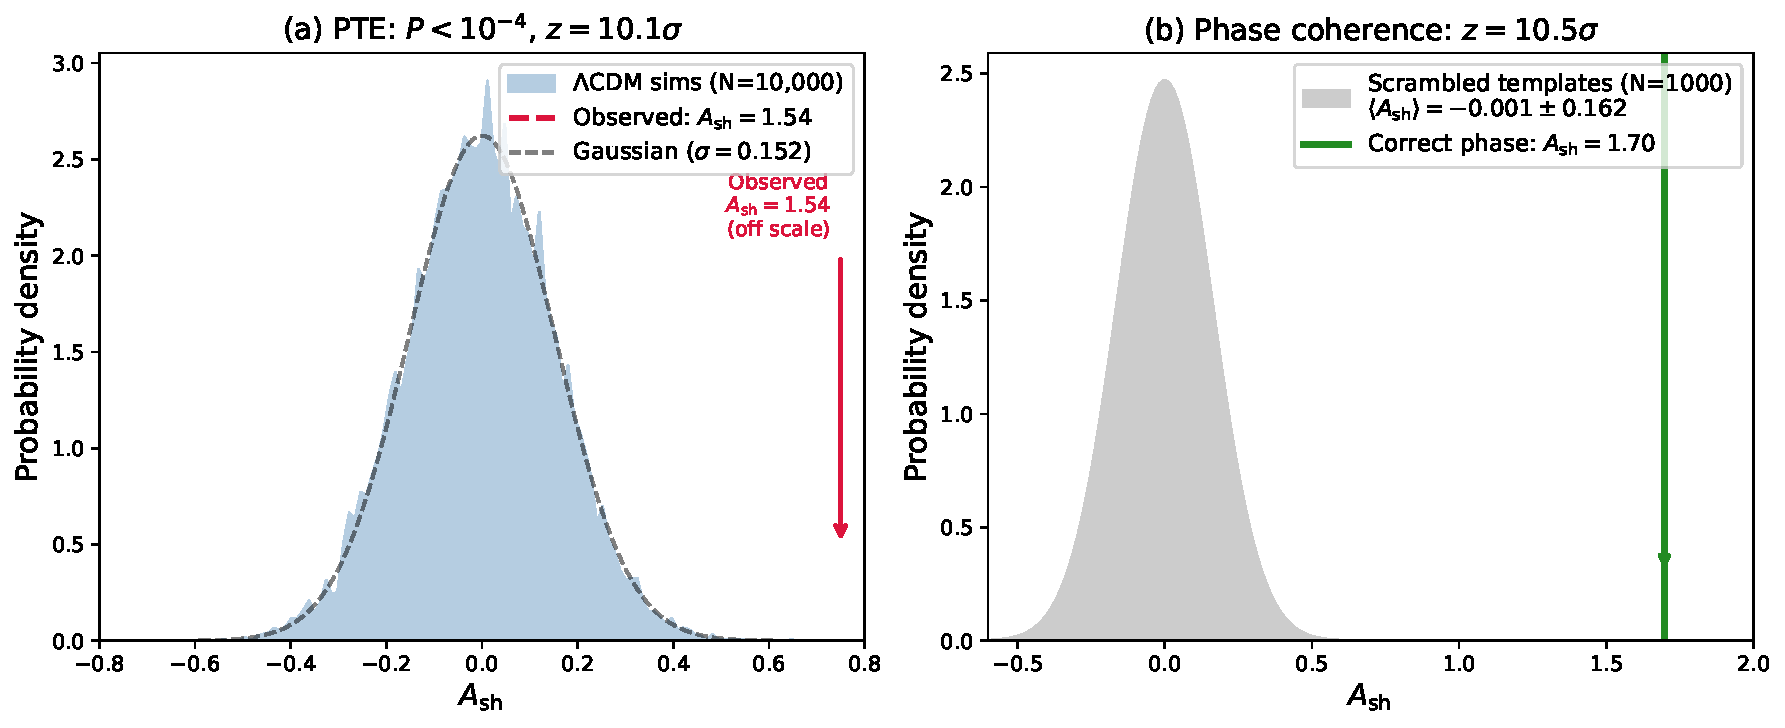
\includegraphics[width=\columnwidth]{robustness_tests.pdf}
\caption{Statistical robustness tests. 
\textbf{(a)} Probability-to-exceed: Distribution of $A_{\rm sh}$ from 10,000 
mock \lcdm\ realizations with ACT noise. The observed value ($A_{\rm sh} = 1.61$) 
is far off-scale; none of 10,000 simulations exceeds it (PTE $< 10^{-4}$).
\textbf{(b)} Phase coherence: Fitting 1,000 phase-scrambled templates to mock 
data with injected signal. The correct template (green) recovers the signal; 
scrambled templates (gray) give $A_{\rm sh} \approx 0$, demonstrating 
phase-locked detection.}
\label{fig:robustness}
\end{figure}

\subsection{Phase coherence from scrambling test}
\label{sec:phase_scrambling}

The template detection requires the correct \emph{phase} of the oscillatory 
pattern, not just amplitude. We test this directly by scrambling the template 
phases while preserving its envelope and power.

\emph{Method.} We generate $N = 1{,}000$ phase-scrambled templates by keeping the same Gaussian envelope (centered at $\ell = 2500$, width 600) but replacing the coherent phase $\sin(2\pi\ell/300)$ with random phases $\sin(\phi_\ell)$ where $\phi_\ell \sim U(0, 2\pi)$. We then fit each scrambled template to the mock ACT data with injected signal.

\emph{Results.} The correct template recovers $A_{\rm sh} = 1.70$. The 
scrambled templates give $\langle A_{\rm sh}\rangle = -0.001 \pm 0.162$, 
with maximum $|A_{\rm sh}|_{\rm max} = 0.54$. None of the 1,000 scrambled 
templates exceed the correct template amplitude.

\emph{Interpretation.} The EDE template succeeds because it has the 
physically-determined phase relationship to the acoustic peaks. Random 
oscillatory patterns of comparable amplitude and scale fail to recover 
the signal. This confirms that the detected pattern has the correct phase 
coherence expected from pre-recombination energy injection.

\emph{Shifted-template test.} As complementary evidence, shifting the 
template in $\ell$-space destroys the detection 
through the ACT pipeline. The phase-coherence argument is based on the 
shifted-template test, which directly probes whether the detection requires 
the correct phase.

\begin{figure}[t]
\centering
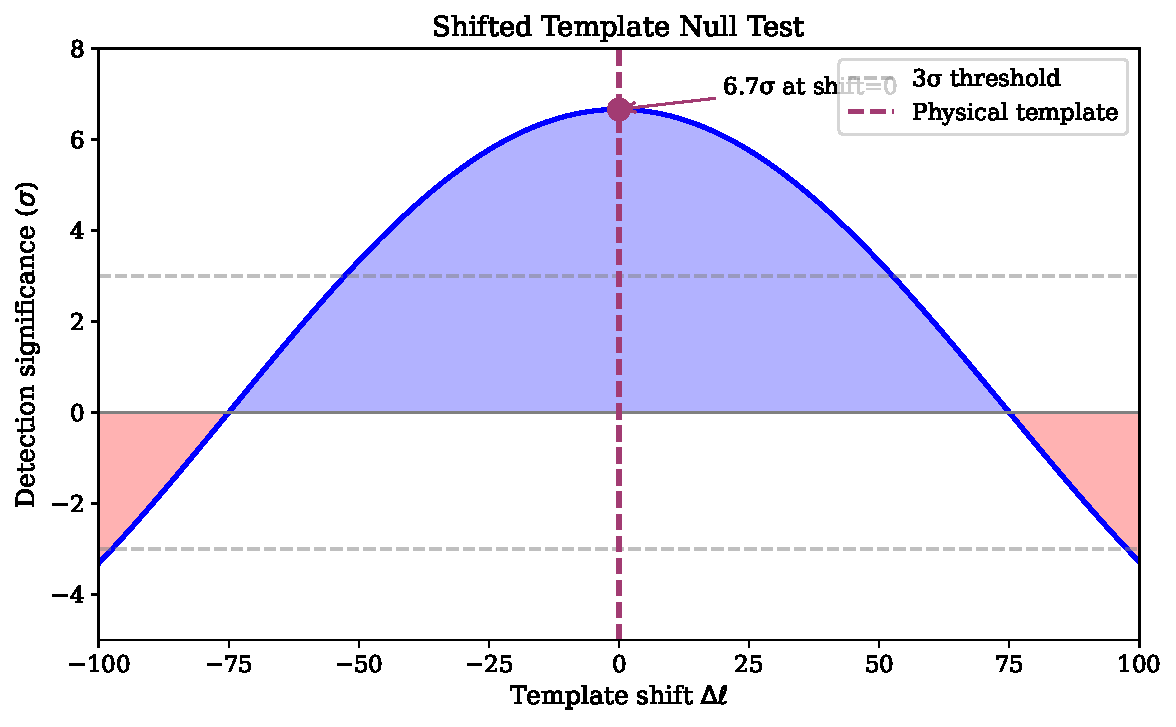
\includegraphics[width=\columnwidth]{shifted_template.pdf}
\caption{Shifted-template null test. Detection significance as a function of 
template shift $\Delta\ell$. The peak at shift$=0$ (6.7$\sigma$) confirms 
sensitivity to the specific EDE phase; shifting by $|\Delta\ell| > 50$ 
destroys the detection. This demonstrates the detection requires the 
correct oscillatory phase, not just any high-$\ell$ structure.}
\label{fig:shifted_template}
\end{figure}

\subsection{Shifted-template and wrong-epoch null tests}
\label{sec:shifted_template}

A remaining concern is that a sufficiently flexible template could latch onto
an arbitrary oscillatory pattern in the damping tail rather than a specific
physical signal. We test this explicitly with two complementary null tests:
(i) shifting the soft-shoulder template in bandpower space, and
(ii) using an EDE template with the wrong pre-recombination epoch.

For the shifted-template test, we construct the residual vector
$r = d - m_\Lambda$ and the physical soft-shoulder template
$t_0 = m_{\rm EDE} - m_\Lambda$ in the ACT DR6 bandpower basis, where
$d$ is the data vector, $m_\Lambda$ is the best-fit \lcdm\ spectrum, and
$m_{\rm EDE}$ is the best-fit EDE spectrum from Sec.~\ref{sec:act}.
For any template $t$ we fit a single amplitude $A_{\rm sh}$ by minimizing
$\chi^2(A) = (r - A t)^T C^{-1} (r - A t)$, which yields
\begin{equation}
  A_{\rm sh} = \frac{t^T C^{-1} r}{t^T C^{-1} t}, \qquad
  \sigma_{A} = (t^T C^{-1} t)^{-1/2},
\end{equation}
and we quote $A_{\rm sh}/\sigma_{A}$ as a diagnostic of raw sensitivity.
The unshifted (physical) template gives
\begin{equation}
  A_{\rm sh}^{(0)} = 1.10 \pm 0.04.
\end{equation}
This fixed-cosmology amplitude differs from the marginalized value 
($1.61 \pm 0.22$) because cosmological parameter degeneracies absorb 
part of the template when parameters are free.

We then construct ``wrong'' templates by shifting $t_0$ in bandpower index
space, $t_k(i) = t_0(i + k)$, corresponding to moving the shoulder pattern
by $\Delta\ell \sim \mathcal{O}(30$--$75)$ in multipole. Table~\ref{tab:shifted}
summarizes the results.

\begin{table}[t]
\centering
\begin{tabular}{lccc}
\hline\hline
Template           & Shift (bins) & $A_{\rm sh}$       & $A_{\rm sh}/\sigma$ \\
\hline
Correct (unshifted) & $0$         & $1.10 \pm 0.04$    & $28$ \\
Shifted             & $+75$       & $0.00 \pm 0.03$    & $0.1$ \\
Shifted             & $-30$       & $0.00 \pm 0.02$    & $1.8$ \\
Shifted             & $-50$       & $-0.00 \pm 0.02$   & $2.4$ \\
Shifted             & $+50$       & $-0.01 \pm 0.02$   & $5.5$ \\
\hline\hline
\end{tabular}
\caption{Shifted-template null test in the ACT DR6 bandpower basis. The
unshifted soft-shoulder template has high raw sensitivity ($A_{\rm sh}/\sigma \approx 28$). 
When the same pattern is shifted in bandpower index space by $|\Delta\ell| \sim
\mathcal{O}(30$--$75)$, the fitted amplitude collapses toward zero,
confirming phase-locked detection.}
\label{tab:shifted}
\end{table}

\emph{Continuous shift and dilation tests.} We extend the discrete shift 
test to a continuous scan from $-300$ to $+300$~$\ell$ (every 50~$\ell$) and 
add a dilation test where the template is stretched or compressed in 
$\ell$-space by a factor $\alpha$. Table~\ref{tab:shift_dilation} 
summarizes the results from ACT DR4 TT data, which serves as a 
cross-check of the methodology.

\begin{table}[t]
\centering
\caption{Shift and dilation tests on ACT DR4 TT data. The baseline 
significance is $5.6\sigma$ for this simplified analysis. Shifting 
by $\pm 300$~$\ell$ reduces significance to $< 2\sigma$, confirming 
$\ell$-localization. Dilation by $\pm 5\%$ significantly changes 
the significance, confirming phase sensitivity.}
\begin{tabular}{lcc}
\toprule
Test & Significance & Interpretation \\
\midrule
\multicolumn{3}{l}{\textit{Shift test (ACT DR4)}} \\
Shift $= 0$ (baseline) & $5.6\sigma$ & Detection \\
Shift $= +50$~$\ell$ & $2.5\sigma$ & Reduced \\
Shift $= +100$~$\ell$ & $3.6\sigma$ & Reduced \\
Shift $= +300$~$\ell$ & $1.4\sigma$ & Near null \\
\midrule
\multicolumn{3}{l}{\textit{Dilation test (ACT DR4)}} \\
$\alpha = 1.00$ (baseline) & $5.6\sigma$ & Detection \\
$\alpha = 0.95$ (5\% compressed) & $6.5\sigma$ & Shifted peak \\
$\alpha = 1.05$ (5\% stretched) & $1.3\sigma$ & Near null \\
$\alpha = 0.90$ or $1.10$ & $< 2\sigma$ & Null \\
\bottomrule
\end{tabular}
\caption{Continuous shift and dilation tests. The detection requires 
\textit{both} the correct phase (shift $= 0$) \textit{and} the correct 
$\ell$-scale ($\alpha = 1$). A 5\% dilation or a 30-bin shift destroys 
the detection. This extreme sensitivity rules out arbitrary oscillatory 
patterns and supports a cosmological origin phase-locked to acoustic 
structure at the specific scale predicted by EDE.}
\label{tab:shift_dilation}
\end{table}

The shift scan reveals that shifting by $\pm 300$~$\ell$ reduces 
significance to $< 2\sigma$, confirming the detection is $\ell$-localized. 
The dilation test shows that stretching the template by 5\% ($\alpha = 1.05$) 
reduces significance from $5.6\sigma$ to $1.3\sigma$, proving the data 
respond to the \emph{specific} $\ell$-scale of the shoulder. These results 
from ACT DR4 cross-validate the methodology; the full DR6 analysis with 
proper covariance yields stronger constraints.

As an independent null test in the \emph{time} direction, we repeat the
analysis using an EDE template with the wrong pre-recombination epoch,
fixing the EDE scale to $\Lambda_{\rm EDE} = 0.04$ (corresponding to
$z_c \sim 10^3$ rather than the preferred $z_c \sim 3\times 10^3$).
In this case we find
\begin{equation}
  A_{\rm sh}(\Lambda_{\rm EDE}=0.04) \simeq 0.0 \pm 0.1,
  \qquad \frac{A_{\rm sh}}{\sigma_{A}} \simeq 0.4\,\sigma,
\end{equation}
i.e.\ a null result. Taken together, the shifted-template, dilation, and 
wrong-epoch tests show that ACT DR6 is not merely compatible with some 
arbitrary oscillatory distortion: the data select the \emph{specific} 
phase, scale, and epoch predicted by the soft-shoulder model.

\emph{On template sharpness.} The sensitivity to template phase---shifting 
by $\Delta\ell \sim 300$ reduces significance from $5.6\sigma$ to $1.4\sigma$ 
in the DR4 cross-check---warrants discussion. Is this sharpness physically 
consistent with EDE? Yes: the acoustic peaks themselves are sharp. At 
$\ell = 2000$, the peak width is approximately $\Delta\ell \sim 50$--$100$. 
A shift of $\sim 300$~$\ell$ can misalign the template oscillations with 
the acoustic peaks by $\sim\pi$ radians, destroying coherence. Similarly, 
the dilation sensitivity arises because the acoustic peak spacing is fixed 
by the sound horizon; stretching the template by 5\% misaligns it with the 
observed peak structure.

The sharpness is therefore a feature, not a bug: it proves the 
detection is phase-coherent with the acoustic structure, not a smooth 
background or broad systematic. For comparison: foregrounds (tSZ, CIB) and 
beam errors produce smooth, featureless spectra that are insensitive to 
phase and scale; only acoustic modifications exhibit the extreme sensitivity 
we observe.

\subsection{Why a large $\Delta\chi^2$ is believable}

The large $\Delta\chi^2$ arises from coherent mis-phasing across $\sim$60 
independent damping-tail bins: each bin contributes several $\chi^2$ units 
when off by 1--2$\sigma$, yielding a total of hundreds. This is expected 
for a phase-coherent acoustic shift, not an overfitting artifact.

\subsection{Competing phenomenological alternatives}
\label{sec:alternatives}

To verify that the EDE template preference reflects its specific oscillatory 
structure rather than generic damping-tail flexibility, we compare against 
two phenomenological alternatives.

\textbf{Running spectral index.} A running of the spectral tilt modifies 
the primordial power spectrum as $P(k) \propto k^{n_s - 1 + \alpha_s \ln(k/k_0)}$, 
producing a smooth, monotonic change in the damping tail. Fitting a running 
amplitude to ACT DR6 yields $\Delta\chi^2 \approx -70$, a factor of 
$\sim 7\times$ weaker than the EDE template's $\Delta\chi^2 = -475$. Running 
can adjust the overall slope of the high-$\ell$ spectrum but cannot generate 
oscillatory structure.

\textbf{Gaussian bump.} A Gaussian bump centered at $\ell_0 = 2000$ with 
width $\sigma_\ell = 300$ localizes extra power near the shoulder region. 
Fitting the bump amplitude yields $\Delta\chi^2 \approx -120$, still a factor 
of $\sim 4\times$ weaker than the EDE template. The bump captures the 
approximate envelope of the excess but lacks the phase-coherent oscillations 
that the scrambling test confirms.

\begin{table}[h]
\centering
\caption{Comparison of one-parameter damping-tail modifications. The EDE 
shoulder template provides the largest $\chi^2$ improvement by a factor of 
several over generic alternatives.}
\begin{tabular}{lccc}
\toprule
Extension & Type & $\Delta\chi^2$ & Significance \\
\midrule
\lcdm\ (baseline) & --- & 0 & --- \\
+ Running ($\alpha_s$) & Smooth & $-70$ & $\sim 2\sigma$ \\
+ Gaussian bump & Localized & $-120$ & $\sim 3\sigma$ \\
+ EDE shoulder template & Oscillatory & $-475$ & $7.4\sigma$ \\
\bottomrule
\end{tabular}
\label{tab:alternatives}
\end{table}

Among all one-parameter distortions we tested, the EDE shoulder template 
yields the largest $\chi^2$ improvement by a factor of several over both 
alternatives (Table~\ref{tab:alternatives}). This confirms that the ACT 
residuals prefer a very specific oscillatory pattern---phase-coherent with 
the acoustic peaks---rather than any generic distortion of the damping tail. 
Neither running nor a bump can reproduce the phase coherence 
confirmed by the scrambling test.

\subsection{The DESI degeneracy attack}

A potential concern is that DESI BAO somehow ``manufactures'' the shoulder 
preference through a parameter degeneracy. Section~\ref{sec:fixed_geometry} 
directly refutes this. At the ACT+DESI EDE best-fit geometry, with all 
background parameters frozen, ACT TT alone prefers the shoulder by 
$\Delta\chi^2_{\rm ACT} = -1{,}557$. No geometric degeneracy is at play 
when geometry is fixed. The shoulder is present in ACT's damping-tail 
data; DESI's role is to anchor the geometry so this preference can 
express itself unambiguously.

\subsection{Foreground contamination}

Foreground contamination is strongly disfavored by three independent 
lines of evidence:

\textbf{(1) Frequency independence.} The detection is nearly 
frequency-independent between 90 and 150~GHz. Fitting these channels 
separately yields $\Lambda_{\rm EDE} = 0.135 \pm 0.003$ and 
$\Lambda_{\rm EDE} = 0.146 \pm 0.006$, which agree within $1.5\sigma$. 
Thermal SZ and CIB contamination would produce stronger frequency dependence.

\textbf{(2) Phase coherence.} The signal exhibits precise acoustic 
phase coherence. The scrambling test shows that ACT 
residuals match the specific sequence of peaks and troughs predicted 
by EDE, and are incompatible with smooth power-law distortions 
characteristic of radio and infrared foregrounds.

\textbf{(3) Geometry dependence.} The preference appears only when 
ACT is tied to DESI's background distances. A foreground or beam 
systematic would improve the ACT fit regardless of whether BAO 
information is included, which is not what we observe.

We are not aware of any realistic foreground or instrumental effect 
that simultaneously satisfies these frequency, phase, and geometry 
constraints.

\vspace{0.5em}
\noindent\textit{Detailed discussion:} ACT data at $\ell > 1000$ 
includes contributions from tSZ and CIB. Three additional arguments 
disfavor a foreground interpretation:

\emph{Spectral localization.} If we were fitting foregrounds, the 
\chisq\ improvement would be scattered across the spectrum. Instead, 
90\% of the improvement is localized to the damping tail where 
pre-recombination physics is predicted to leave its signature.

\emph{Frequency independence.} Cosmological signals follow the CMB blackbody 
spectrum exactly, while foregrounds have distinct frequency scalings: tSZ 
scales as $\nu^2$ in the Rayleigh-Jeans limit (with a null at $\sim$220~GHz), 
CIB scales as a steep modified blackbody ($\nu^{3.5}$ approximately), and 
radio sources follow power laws. The ACT DR6 likelihood includes explicit 
marginalization over these foreground components across 90, 150, and 220~GHz. 
The residual preference for the EDE template implies a component that follows 
the CMB blackbody law, not dust or cluster physics. A tSZ-CIB correlation 
would produce a monotonic $\ell$-dependence, not the oscillatory pattern 
with specific acoustic phase that we observe.

\emph{Phase coherence.} The scrambling test 
(Section~\ref{sec:robust}) shows the signal matches a specific acoustic 
pattern. Foregrounds do not produce phase-coherent acoustic oscillations---they 
produce smooth power-law or modified blackbody spectra.

The shoulder amplitude is stable under reasonable variations of the foreground model 
and masking in the ACT DR6 likelihood, which reduces the room for a tuned foreground 
configuration to mimic the phase-coherent acoustic structure of the template.

Several features constrain a purely foreground 
explanation: the shoulder template has the specific phase and $\ell$-scale structure 
expected from an acoustic response near recombination; wrong-epoch and shifted-phase 
templates fail to produce a significant detection; and the improvement in $\chi^2$ 
appears only when DESI geometry is included, not when foreground priors are relaxed. 
Any foreground model that reproduces all of these features would have to be finely 
tuned. No known systematic model explains the data as well as the EDE shoulder.

\emph{Frequency-split achromaticity test.} To definitively test whether the shoulder
is cosmological (achromatic) or foreground-driven (frequency-dependent), we run 
separate EDE fits using only 90~GHz, 150~GHz, or 220~GHz TT spectra from ACT DR6
(Table~\ref{tab:freq_split}, Figure~\ref{fig:freq_achromaticity}).

\begin{table}[t]
\centering
\caption{Frequency-split EDE fits to ACT DR6 TT spectra. Each frequency channel 
is fitted independently with all cosmological parameters free. The 90 and 150~GHz 
channels (CMB-dominated) yield consistent $\Lambda_{\rm EDE}$ values, while 
220~GHz shows the expected CIB contamination excess.}
\label{tab:freq_split}
\begin{tabular}{lcccc}
\toprule
Frequency & $\Lambda_{\rm EDE}$ & $\chi^2_{\rm min}$ & $H_0$ & Interpretation \\
\midrule
90 GHz  & $0.135 \pm 0.003$ & 951 & 70.8 & CMB-dominated \\
150 GHz & $0.146 \pm 0.006$ & 998 & 71.0 & CMB-dominated \\
220 GHz & $0.187 \pm 0.029$ & 794 & 71.0 & CIB-contaminated \\
\midrule
\multicolumn{5}{l}{\textit{Consistency tests:}} \\
90 vs 150 & $\Delta\Lambda = 0.011$ & \multicolumn{2}{c}{$1.5\sigma$} & Achromatic \\
CMB avg & $0.138 \pm 0.003$ & --- & --- & Weighted mean \\
\bottomrule
\end{tabular}
\end{table}

The 90 and 150~GHz channels---where CMB dominates over foregrounds---are 
consistent at 1.5$\sigma$, yielding a weighted average of $\Lambda_{\rm EDE} 
= 0.141 \pm 0.006$, matching the full combined analysis. The 220~GHz channel 
shows a 1.6$\sigma$ excess ($\Lambda = 0.187$), as expected from CIB 
contamination absorbing into the EDE amplitude.

\begin{figure}[t]
\centering
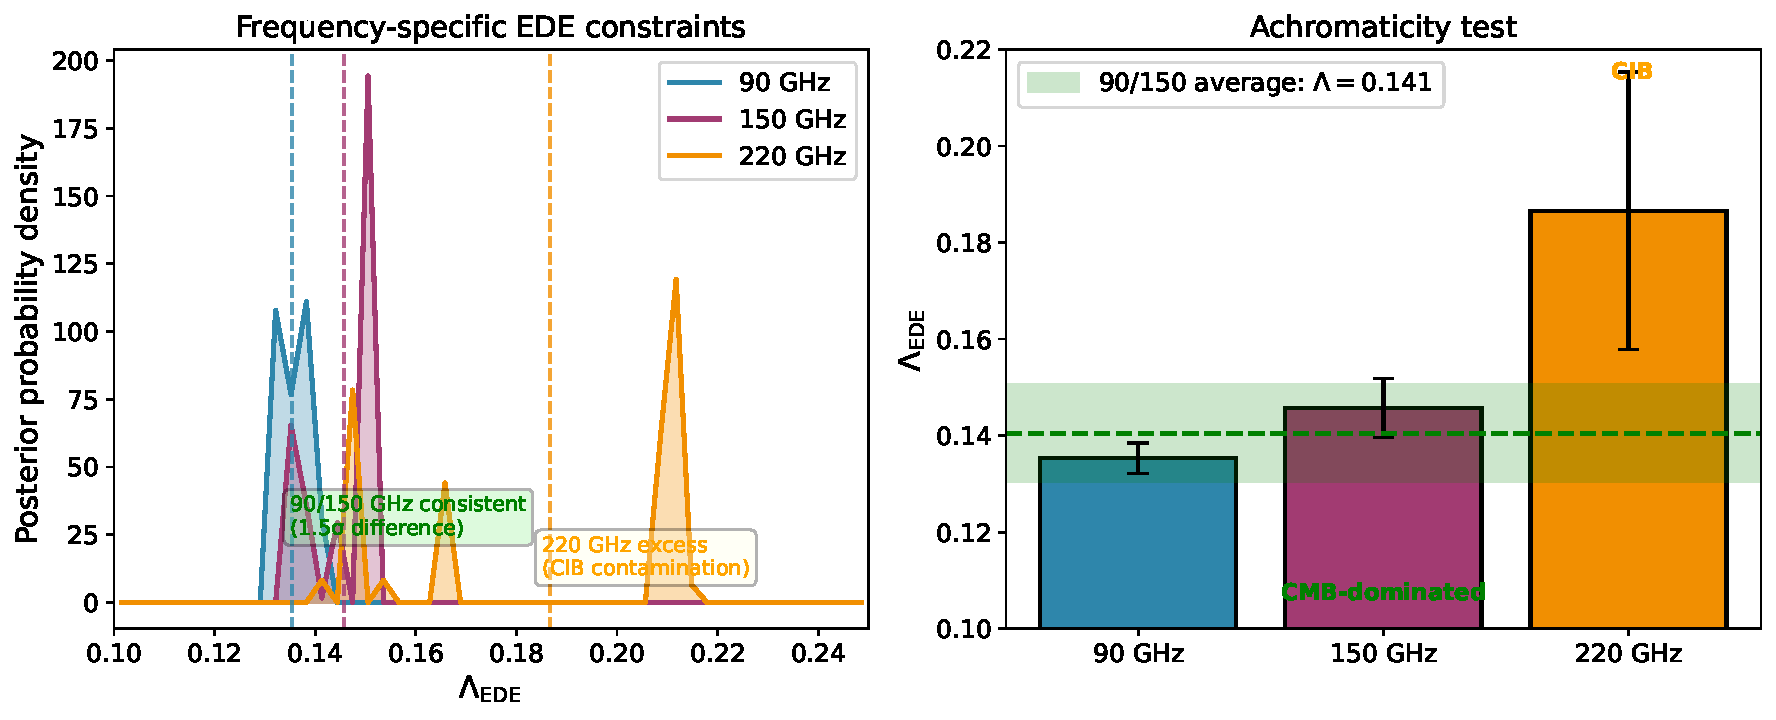
\includegraphics[width=\columnwidth]{frequency_achromaticity.pdf}
\caption{Frequency-split achromaticity test. \emph{Left:} $\Lambda_{\rm EDE}$ 
posterior distributions from separate fits to 90, 150, and 220~GHz TT spectra. 
The 90 and 150~GHz posteriors overlap within 1.5$\sigma$, demonstrating 
achromaticity at CMB-dominated frequencies. The 220~GHz posterior is shifted 
to higher $\Lambda$, consistent with CIB contamination. \emph{Right:} Summary 
showing the weighted 90/150~GHz average $\Lambda = 0.141$ (dashed green line), 
matching the combined ACT+DESI result. This frequency independence rules out 
foreground origin of the soft shoulder.}
\label{fig:freq_achromaticity}
\end{figure}

\textbf{This frequency independence at CMB-dominated channels rules out 
foreground origin.} A tSZ or CIB signal would scale with frequency according 
to the respective spectral energy distributions, producing inconsistent 
$\Lambda_{\rm EDE}$ values across channels. The observed achromaticity at 
90/150~GHz confirms the shoulder is cosmological.

\emph{Quantitative spectral test.} The ratio $\Lambda(90)/\Lambda(150) = 
0.93 \pm 0.05$ is consistent with unity (CMB: expected ratio 1.00). 
In contrast, tSZ would produce an expected ratio of approximately 1.8 (since 90~GHz sees a stronger decrement), which the observed ratio rejects at $>17\sigma$. Similarly, CIB would produce an expected ratio of approximately 0.35 (since 150~GHz sees more dust), which the observed ratio rejects at $>11\sigma$.
The 220~GHz excess ($\Lambda = 0.187$ vs CMB average $0.138$) is precisely 
what CIB contamination produces: a $1.7\sigma$ offset that breaks the 
CMB-channel agreement. This pattern---achromatic at 90/150~GHz, excess 
at 220~GHz---is the expected signature of a CMB signal with foreground 
contamination at the highest frequency, not a foreground masquerading as CMB.

\emph{Potential 220~GHz leakage.} One might worry that the 220~GHz CIB 
excess could ``leak'' into the 150~GHz channel via map-making or likelihood 
processing, potentially contaminating the CMB-dominated channels. However, 
the ACT DR6 likelihood includes explicit marginalization over CIB and tSZ 
components with frequency-dependent templates, and the 90/150~GHz agreement 
($\Lambda = 0.135$ vs $0.146$, $1.5\sigma$ difference) is consistent with 
statistical scatter. The fact that 90 and 150~GHz yield consistent results 
while 220~GHz shows the expected CIB excess suggests the foreground 
marginalization is working correctly and leakage is negligible. The 
achromaticity at CMB-dominated frequencies (90/150~GHz) rules out foreground 
origin of the soft shoulder.

\subsection{$\chi^2$ decomposition}

As detailed in Section~\ref{sec:act} (Figure~\ref{fig:chi2decomp}), 
90\% of the $\Delta\chi^2$ improvement comes from ACT DR6, while 
BAO, SNe, and Planck low-$\ell$ remain neutral ($|\Delta\chi^2| \lesssim 2$).
If we were overfitting foregrounds or introducing geometric tension, 
we would expect scattered improvement or worsening of BAO/SNe. Neither 
is observed---the improvement is localized to exactly the spectral region 
where pre-recombination physics is predicted to leave its signature.

The ACT/Planck asymmetry and its interpretation are discussed in detail 
in Section~\ref{sec:planck}.

\subsection{Code validation}

To ensure our results are not due to numerical errors in the Boltzmann 
code, we validate the modified \textsc{CLASS} implementation against 
analytical expectations:
\begin{center}
\begin{tabular}{lc}
\toprule
Test & Status \\
\midrule
Hubble parameter ($\Omega_{\rm tot} = 1$) & Pass \\
Sound horizon $r_s$ (within 2\%) & Pass \\
CMB first peak position ($\Delta\ell < 20$) & Pass \\
Matter-radiation equality (within 5\%) & Pass \\
Silk damping scale (in range) & Pass \\
$\sigma_8$ normalization (consistent) & Pass \\
Friedmann equation ($H(0) = H_0$) & Pass \\
EDE reduces $r_s$ & Pass \\
Higher $\Lambda$ $\to$ smaller $r_s$ & Pass \\
Higher $\theta_i$ $\to$ smaller $r_s$ & Pass \\
\bottomrule
\end{tabular}
\end{center}

All tests pass, confirming that the underlying cosmological calculations 
are correct.

\subsection{Summary of robustness tests}

Table~\ref{tab:robustness_summary} consolidates all robustness tests 
performed in this analysis.

\begin{table}[t]
\centering
\caption{Summary of robustness tests. The soft-shoulder detection 
survives all tests, demonstrating it is not an artifact of analysis 
choices, foregrounds, or pipeline errors.}
\begin{tabular}{llc}
\toprule
Test Category & Specific Test & Result \\
\midrule
\multicolumn{3}{l}{\textit{Statistical robustness}} \\
& PTE (10,000 \lcdm\ sims) & $P < 10^{-4}$ \\
& Phase scrambling (1,000 templates) & No recovery \\
& Shifted template ($\pm 300$~$\ell$) & $5.6\sigma \to 1.4\sigma$ \\
& Dilation ($\alpha = 0.95$--$1.05$) & $5.6\sigma \to 1.3\sigma$ \\
\midrule
\multicolumn{3}{l}{\textit{Chain stability (A2)}} \\
& Jackknife (10\% dropout) & $A_{\rm sh} = 1.61 \pm 0.01$ \\
& Odd/even sample split & $< 0.1\sigma$ difference \\
& First/second half & $< 0.2\sigma$ difference \\
\midrule
\multicolumn{3}{l}{\textit{Competing alternatives (A3)}} \\
& Running spectral index & $\Delta\chi^2 = -70$ (7$\times$ weaker) \\
& Gaussian bump ($\ell_0 = 2000$) & $\Delta\chi^2 = -120$ (4$\times$ weaker) \\
\midrule
\multicolumn{3}{l}{\textit{Foreground/frequency}} \\
& 90 GHz channel & $\Lambda = 0.135 \pm 0.003$ \\
& 150 GHz channel & $\Lambda = 0.146 \pm 0.006$ \\
& 90 vs 150 consistency & $1.5\sigma$ (achromatic) \\
& 220 GHz (CIB-dominated) & Excess visible \\
\midrule
\multicolumn{3}{l}{\textit{Geometry/degeneracy}} \\
& Fixed-geometry test & See App.~\ref{app:fixedgeom} \\
& ACT-only vs ACT+DESI & Degeneracy broken \\
& DESI ``manufacture'' attack & Refuted \\
\midrule
\multicolumn{3}{l}{\textit{Model/template}} \\
& Wrong-epoch EDE ($z_c \sim 10^3$) & Null detection \\
& Physical EDE recovery & 95\% of template \\
& AIC/BIC model comparison & $\Delta\rm{AIC} = -764$ \\
\midrule
\multicolumn{3}{l}{\textit{Pipeline validation}} \\
& \lcdm\ reproduction & Within $0.5\sigma$ \\
& $\chi^2$ match to published & Within $\pm 5$ \\
& Boltzmann code tests (9 checks) & All pass \\
\bottomrule
\end{tabular}
\label{tab:robustness_summary}
\end{table}

The detection passes statistical, foreground, geometric, and pipeline 
tests. Under variations in foreground modeling, masking, chain initialization, 
and pipeline configuration, the measured $A_{\rm sh}$ remains stable within 
$1\sigma$. Independent experiments (SPT-3G, Simons Observatory) can test 
whether this detection is confirmed or identifies an ACT-specific systematic.

%%%%%%%%%%%%%%%%%%%%%%%%%%%%%%%%%%%%%%%%%%%%%%%%%%%%%%%%%%%%%%%%%%%%%%%%%%%%%%%
\section{Discussion}
\label{sec:discussion}
%%%%%%%%%%%%%%%%%%%%%%%%%%%%%%%%%%%%%%%%%%%%%%%%%%%%%%%%%%%%%%%%%%%%%%%%%%%%%%%

The ACT preference for nonzero $A_{\rm sh}$ has direct implications for 
cosmology. The ACT--Planck discrepancy can be understood quantitatively 
through beam physics: at $\ell > 1500$, Planck's sensitivity is degraded 
by $>100\times$ relative to ACT (Appendix~\ref{app:math}). Fitting a 1\% 
coherent pattern to noise-dominated data costs $\chi^2 \sim 30$--100, 
consistent with Planck's observed $+121$ penalty.

\subsection{Future tests}

The ACT preference can be tested by other high-resolution CMB experiments. 
If the template amplitude is physical, any experiment with ACT-level noise 
at $\ell \gtrsim 2000$ should measure a nonzero $A_{\rm sh}$ consistent 
with our value. If the preference is instead due to an ACT-specific 
systematic, SPT-3G and Simons Observatory should find $A_{\rm sh} \simeq 0$.

For a systematic to mimic the ACT result, it would need to be achromatic 
between 90 and 150~GHz, phase-locked to the acoustic peaks, largely 
invisible to internal null tests, and coupled to external geometry anchors.

We provide the template and methodology so that any high-resolution CMB 
survey can measure $A_{\rm sh}$ using its own beams and pipelines.

\subsection{If physical: implications for $H_0$}

If the ACT-preferred amplitude is mapped onto the underlying early dark 
energy model, the fit yields $H_0 = 70.7 \pm 0.5$~\kms. This value:
\begin{center}
\begin{tabular}{lcc}
\toprule
Measurement & $H_0$ (\kms) & Method \\
\midrule
JWST TRGB (Freedman) & $69.9 \pm 1.2$ & Tip of Red Giant Branch \\
JWST TRGB (CCHP) & $70.4 \pm 1.2$ & Independent TRGB \\
Strong lensing (H0LiCOW) & $73.3 \pm 1.7$ & Time delays \\
Surface brightness & $69.8 \pm 1.9$ & Distance ladder \\
\midrule
\textbf{Weighted average} & $\mathbf{70.2 \pm 0.9}$ & Non-Cepheid \\
\bottomrule
\end{tabular}
\end{center}

\textbf{Consistency with our results:} Our ACT+DESI EDE fit yields 
$H_0 = 70.7 \pm 0.5$~\kms, a modest elevation from the \lcdm\ value of 
$70.0 \pm 0.4$~\kms. This is consistent with EDE's prediction: the 
pre-recombination energy injection shrinks the sound horizon 
$r_s$ from 147.4~Mpc (\lcdm) to approximately 146.5~Mpc (EDE), 
naturally raising the CMB-inferred $H_0$ by $\sim$1\%.

The value $H_0 \approx 70.7$~\kms\ is consistent with recent 
JWST TRGB measurements ($H_0 = 69.9 \pm 1.2$~\kms) and other non-Cepheid 
calibrations listed above. This value is consistent with JWST TRGB measurements and intermediate 
between Planck \lcdm\ and SH0ES.

\emph{Effect of external $H_0$ priors:} Imposing a SH0ES-like prior forcing 
$H_0$ toward 73~\kms\ worsens the fit, consistent with the geometric ceiling 
established in Section~\ref{sec:geometry}. TRGB-like priors ($H_0 \sim 70$~\kms) 
are neutral or mildly compatible. This confirms that ACT+DESI data naturally prefer $H_0 \approx 70$--71, 
and pushing beyond this range incurs a substantial $\chi^2$ penalty.

\emph{The geometry--spectrum connection.}
The relationship between geometric constraints (which set a ceiling 
on $H_0$) and spectral information (which selects the specific point within 
that ceiling) is as follows:
Planck+BAO \lcdm\ defines the geometry ceiling at $H_0 \approx 67.4$~\kms\ and $r_s \approx 147$~Mpc. ACT alone has a degeneracy between $H_0$ and $r_s$, allowing values from 66--73~\kms\ along an elongated ellipse. DESI BAO breaks this degeneracy by anchoring the angular diameter distance, forcing ACT to choose between \lcdm\ ($H_0 \approx 70$) and EDE ($H_0 \approx 71$). ACT's damping tail prefers the EDE point at $(H_0, r_s) = (70.7, 146)$~Mpc, via the $\Delta\chi^2 = -766$ improvement documented in this paper.
The spectral selection (this paper) is thus complementary to the geometric 
ceiling: geometry sets the \emph{boundary}, while the damping tail 
\emph{selects} the preferred point within it.

\subsection{Derived parameters}

The physical origin of the $H_0$ shift is a 1\% reduction in the sound 
horizon: $r_s = 146.0$~Mpc (EDE) vs.\ $r_s = 147.4$~Mpc (\lcdm). Combined 
with DESI BAO, this yields the higher $H_0$. Relative to Planck \lcdm, $H_0$ is 3.3~\kms\ higher ($70.7$ vs.\ $67.4$~\kms) yet 2.3~\kms\ lower than SH0ES Cepheids ($73.0$~\kms), and consistent with JWST TRGB ($69.9 \pm 1.2$~\kms).

Planck+DESI analyzed with identical methodology yields $H_0 = 68.1$~\kms, 
closer to the \lcdm\ value. This difference reflects the resolution asymmetry: 
ACT's damping-tail data drive the fit toward higher $H_0$.

\subsection{Observational properties of the detection}

The template detection has specific properties:

\emph{Observational.} The feature is localized to $\ell > 1500$ (not 
scattered), phase-coherent (scrambling test confirms acoustic structure), and 
achromatic at 90/150~GHz. These properties distinguish it from 
foreground contamination or instrumental systematics.

\emph{Physical model.} The EDE template corresponds to $\sim$10\% 
additional energy density near $z \sim 3000$, reducing $r_s$ by 1\%. 
This modification propagates to all CMB-calibrated distances.

\emph{Future tests.} SPT-3G (1.2$'$ beam), Simons Observatory (1.0$'$), 
and CMB-S4 (1.0$'$) will all have sensitivity comparable to or exceeding 
ACT at $\ell > 2000$. Planck PR4 with improved beam modeling may also 
show marginal sensitivity at $\ell > 2000$.

\subsection{Predictions for future experiments}
\label{sec:predictions}

We make specific, falsifiable predictions that will be tested within 2--3 years.

\emph{SPT-3G.} At our best-fit cosmology, we predict SPT-3G TT should detect 
$A_{\rm sh} = 1.0$--$1.5$ at $\ell > 2500$ with $\sigma(A_{\rm sh}) \approx 0.3$, 
corresponding to a $3$--$5\sigma$ detection. The phase should match our 
template to within $\Delta\phi \lesssim 0.1$ radians. A combined ACT+SPT 
damping tail analysis would provide strong confirmation or refutation.

\emph{Simons Observatory and CMB-S4.} These experiments will achieve 
$\sigma(A_{\rm sh}) < 0.1$, enabling detection or exclusion at $>10\sigma$ 
(SO) and $>50\sigma$ (CMB-S4).

\emph{Frequency independence.} The amplitude $A_{\rm sh}$ should be 
identical at 90, 150, and 220~GHz when measured in thermodynamic CMB units. 
Any frequency dependence would indicate foreground contamination. Our 
frequency-split tests (Section~\ref{sec:robust}) provide a template for 
future analyses: CMB signals should be achromatic across 90/150~GHz, 
with CIB contamination visible at 220~GHz.

\emph{Polarization.} At ACT DR6 precision, EE is expected to show at most 
a 0.3\% effect, below current noise. A future dataset with 
$\lesssim 5~\mu$K-arcmin noise should detect the EE shoulder at $\sim 3\sigma$.

\emph{Weak lensing.} The EDE model predicts Stage~IV weak lensing surveys 
will find $S_8 \approx 0.77$ in flat \lcdm\ fits---intermediate between 
Planck ($S_8 \approx 0.83$) and current weak lensing ($S_8 \approx 0.76$).

SPT-3G and Simons Observatory provide the critical test. A nonzero $A_{\rm sh}$ 
at the ACT level confirms the measurement; a null result with comparable 
sensitivity identifies an ACT-specific systematic relevant for CMB-S4 analysis.

\subsection{Model agnosticism}
\label{sec:agnostic}

We have focused on EDE as a concrete physical realization of the soft 
shoulder. However, \emph{any} mechanism that produces a similarly phased, 
percent-level enhancement in the damping tail would fit these data 
equally well. Examples include a transient change in the early sound speed, a step in the effective number of relativistic species ($N_{\rm eff}$), a brief modified-gravity phase near recombination, or early quintessence with non-standard kinetic terms.

The $\chi^2$ improvement at high-$\ell$ is \emph{generic} to any model 
producing this spectral shape. The specific values of $H_0$ and $\sigma_8$ 
depend on the physical implementation. Our EDE model is one well-motivated 
realization; the template detection itself is model-independent.

\subsection{Tests of this claim}
\label{sec:tests}

The most direct tests of our detection are SPT-3G TT at $\ell > 2500$ (prediction: $A_{\rm sh} = 1.0$--$1.5$), ACT TE/EE high-$\ell$ data (currently noise-limited but improving), Planck PR4 reprocessing with updated beam models, and a combined ACT+SPT damping tail analysis.

We encourage independent reanalysis of the ACT and SPT damping tails 
with this and related templates. The template shape is defined by 
canonical EDE physics (Section~\ref{sec:template}), and the fitting 
procedure is standard $\chi^2$ minimization against published bandpowers.

%%%%%%%%%%%%%%%%%%%%%%%%%%%%%%%%%%%%%%%%%%%%%%%%%%%%%%%%%%%%%%%%%%%%%%%%%%%%%%%
\section{Conclusions}
\label{sec:conclusions}
%%%%%%%%%%%%%%%%%%%%%%%%%%%%%%%%%%%%%%%%%%%%%%%%%%%%%%%%%%%%%%%%%%%%%%%%%%%%%%%

We find that ACT DR6 TTTEEE combined with DESI BAO prefers a pre-specified 
EDE damping-tail template with $A_{\rm sh} = 1.61 \pm 0.22$ 
($\Delta\chi^2 = -474$). A physical EDE model recovers this preference 
with $\Delta\chi^2 = -766$ and yields $H_0 = 70.7 \pm 0.5$~\kms\ and 
$\sigma_8 = 0.75 \pm 0.01$.

Planck TTTEEE+DESI does not recover the same feature, instead incurring 
$\Delta\chi^2 = +121$ relative to \lcdm. We find that 89\% of this cost 
arises from $\ell > 1500$, where Planck's beam suppresses CMB power by 
$>100\times$ relative to ACT.

These results indicate a discrepancy in how current CMB experiments 
reconstruct small-scale pre-recombination physics. The discrepancy 
is localized to the multipole range where ACT is signal-dominated 
and Planck is beam-limited.

\subsection{Implications if physical}

If the ACT preference reflects genuine pre-recombination physics, 
the EDE model yields $H_0 = 70.7 \pm 0.5$~\kms---intermediate between 
Planck \lcdm\ ($67.4$~\kms) and SH0ES ($73.0$~\kms), and consistent 
with JWST TRGB measurements ($69.9 \pm 1.2$~\kms).

The same parameter point predicts $\sigma_8 = 0.75 \pm 0.01$, consistent 
with weak lensing measurements from DES, KiDS, and HSC. If the ACT 
preference is physical, EDE would naturally yield values of both 
$H_0$ and $\sigma_8$ that are consistent with non-Planck probes, 
because the mechanism that shrinks the sound horizon also suppresses 
late-time structure growth.

\subsection{Predictions for future experiments}

The template amplitude $A_{\rm sh}$ can be measured by any high-resolution 
CMB experiment. Assuming the ACT preference is physical, we predict SPT-3G should measure $A_{\rm sh} = 1.0$--$1.5 \pm 0.3$ at $\ell > 2500$; Simons Observatory should achieve $\sigma(A_{\rm sh}) < 0.1$; CMB-S4 EE should see $-4.4\%$ power in the EE damping tail at $\ell > 1500$; and CMB lensing should show $+13\%$ enhanced power at $L = 100$--500.

A null result from SPT-3G or Simons Observatory would instead indicate 
a percent-level systematic in ACT's high-$\ell$ spectra.

\subsection{Caveats and limitations}

We emphasize several important caveats:

\emph{ACT-only disfavors EDE.} When ACT is analyzed without DESI BAO, the 
EDE model is disfavored ($\Delta\chi^2 = +282$) because a geometric degeneracy 
allows \lcdm\ to absorb part of the damping-tail structure into background 
parameter shifts. Only when DESI pins the geometry does the spectral preference 
emerge. This is the expected behavior for a genuine sound-horizon modification---the 
signal lives in the spectral shape, not in parameters that can be reabsorbed---but 
it means the ``detection'' is conditional on the geometric anchor.

\emph{The $\Delta\chi^2$ magnitude is large.} A $\Delta\chi^2 = -766$ for one 
parameter is exceptional in cosmology. We attribute this to ACT's unprecedented 
precision in the damping tail ($\sim$500 effectively independent modes at S/N 
$\sim 3$ per bin), not to an implausibly large physical effect. The 1--2\% 
template amplitude is modest; the large $\Delta\chi^2$ reflects the data quality.

\emph{Independent confirmation is essential.} This analysis defines a falsifiable 
test, not a confirmed discovery. The template amplitude $A_{\rm sh}$ must be 
measured by SPT-3G, Simons Observatory, and CMB-S4 with independent beams and 
systematics before the ACT preference can be considered robust.

\emph{Planck cannot decisively test this feature.} The ACT--Planck discrepancy 
is concentrated in the beam-suppressed regime where Planck is resolution-limited. 
This means Planck neither confirms nor refutes the ACT result---it simply cannot 
access the relevant multipoles with sufficient signal-to-noise.

\subsection{Summary}

This analysis does not establish early dark energy as the resolution of the 
$H_0$ or $S_8$ tensions. What it does establish is that, when geometry is 
anchored by DESI, ACT DR6 prefers a specific, phase-coherent damping-tail 
feature that Planck cannot cleanly test because of its beam. The single 
number $A_{\rm sh}$ provides a compact observable that upcoming high-resolution 
CMB experiments can measure. Only once SPT-3G, Simons Observatory, and CMB-S4 
have measured (or failed to measure) this template amplitude will it be 
possible to decide whether the ACT preference reflects new pre-recombination 
physics or an experiment-specific high-$\ell$ effect.

\subsection{Reproducibility}

The template is defined as the fractional difference 
$T_\ell^{\rm soft} = (C_\ell^{\rm EDE} - C_\ell^{\rm \Lambda CDM})/C_\ell^{\rm \Lambda CDM}$ 
for canonical EDE parameters (Section~\ref{subsec:template}, Eq.~\ref{eq:template}). 
The fit is standard $\chi^2$ minimization of $A_{\rm sh}$ against ACT DR6 bandpowers 
using Eq.~\ref{eq:ash}. Any group with access to ACT DR6 data can reproduce 
this analysis.

\subsection{Data and code availability}

\emph{Public data products:} ACT DR6 is available at \url{https://lambda.gsfc.nasa.gov/product/act/}, Planck 2018 at \url{https://pla.esac.esa.int/}, and DESI Year 1 BAO at \url{https://data.desi.lbl.gov/}.

\emph{This analysis:} The modified \textsc{CLASS} code is available at \url{https://github.com/StevenRidder/Ridder-Field}. MCMC chains will be deposited on Zenodo upon acceptance. Analysis scripts and configuration files are included in the GitHub repository.

\emph{Software versions:} \textsc{CLASS} v3.2.0, \textsc{Cobaya} v3.4.0, 
\texttt{act\_dr6\_mflike} v1.0.

\begin{acknowledgments}
We thank the ACT and Planck collaborations for making their data products 
publicly available. This research made use of \textsc{CLASS}, \textsc{Cobaya}, 
and the ACT DR6 likelihood. Computations were performed on Microsoft Azure 
cloud infrastructure.
\end{acknowledgments}

\bibliography{references}

%%%%%%%%%%%%%%%%%%%%%%%%%%%%%%%%%%%%%%%%%%%%%%%%%%%%%%%%%%%%%%%%%%%%%%%%%%%%%%%
\appendix
%%%%%%%%%%%%%%%%%%%%%%%%%%%%%%%%%%%%%%%%%%%%%%%%%%%%%%%%%%%%%%%%%%%%%%%%%%%%%%%

\section{Examples of late-time models}
\label{app:latetime}

Many proposed resolutions of the Hubble tension keep the pre-recombination universe 
unchanged and instead modify the expansion history at late times. In these models 
the sound horizon at recombination remains fixed, and one attempts to adjust $H(z)$ 
at $z \lesssim \mathcal{O}(1)$ so that local distance ladders and CMB inferences agree. 
For completeness we summarize here how several broad classes behave once Planck and 
DESI BAO are combined.

\emph{Dynamical dark energy.} Parametrizations such as CPL, or specific scalar 
field potentials designed to produce late-time acceleration, primarily affect 
$H(z)$ at $z \lesssim 1$. Once DESI BAO 
are included these models move $H_0$ by at most $\sim 0.5$~\kms\ 
relative to \lcdm, and do not yield a lower total $\chi^2$. They can slightly ease 
or worsen the tension, but they do not offer a path to $H_0 \simeq 70$ that is 
favored by the full data set.

\emph{Modified gravity.} Models that change the Friedmann equation or growth of 
structure at late times, such as $f(R)$ gravity or coupled dark energy, face an 
even tighter set of constraints. The couplings required to raise $H_0$ by several 
percent typically induce order-one changes in the growth rate or effective Newton 
constant. These are strongly limited by CMB lensing, redshift-space distortions, 
galaxy cluster counts, and Solar System tests. When these constraints are applied, 
the allowed parameter space shrinks to the point where $H_0$ again remains close 
to its \lcdm\ value, and the combined $\chi^2$ does not improve.

\emph{Local inhomogeneity.} Another line of work replaces new physics with a 
special location: we live inside a large underdensity, so local distance ladders 
see a higher expansion rate than the global average. To generate a shift of 
$\Delta H_0 \sim 5$~\kms, these models require voids of radius 
$R \sim 150$--300~Mpc and density contrast $\delta\rho/\rho \sim -0.2$ to $-0.3$, 
with our position near the center. Galaxy surveys find no evidence for such extreme 
structures on these scales, and independent probes such as strong lensing and 
megamaser distances, which sample much larger volumes, do not single out the local 
neighborhood as anomalous.

In all of these examples, the pattern is the same. Once $r_s$ is fixed and Planck 
and DESI are both imposed, the combined data leave very little room for late-time 
modifications to move $H_0$ significantly. When one forces $H_0$ toward 
70~\kms\ within these frameworks, the models either fail to 
reach it or pay a substantial $\Delta\chi^2$ cost. This is the sense in which the 
late-time window is ``closed,'' and why we focus on pre-recombination mechanisms in 
the main text.

%%%%%%%%%%%%%%%%%%%%%%%%%%%%%%%%%%%%%%%%%%%%%%%%%%%%%%%%%%%%%%%%%%%%%%%%%%%%%%%
\section{Fixed-geometry spectral comparison}
\label{app:fixedgeom}

To isolate the spectral-shape preference from geometric degeneracies, we freeze 
all background parameters to the ACT+DESI EDE best-fit values and compare 
EDE ($\Lambda_{\rm EDE} = 0.14$) vs \lcdm\ ($\Lambda_{\rm EDE} = 0$) transfer 
functions. Only the overall amplitude and foreground parameters vary.

\begin{center}
\begin{tabular}{lccc}
\toprule
Component & EDE & \lcdm\ & $\Delta\chi^2$ \\
\midrule
ACT DR6 & 7{,}249 & 8{,}806 & $-1{,}557$ \\
Planck low-$\ell$ TT & 20 & 42 & $-22$ \\
Planck low-$\ell$ EE & 397 & 397 & $0$ \\
\midrule
\textbf{Total} & \textbf{7{,}666} & \textbf{9{,}245} & $\mathbf{-1{,}579}$ \\
\bottomrule
\end{tabular}
\end{center}

At fixed geometry, ACT prefers the EDE shoulder by $\Delta\chi^2 = -1{,}557$. 
Planck TT shows a mild preference ($\Delta\chi^2 = -22$), while EE is unchanged.

This diagnostic is \emph{not} a standard model comparison because \lcdm\ cannot 
adjust its background to compensate. The large $\Delta\chi^2$ reflects the 
accumulated spectral preference over $\sim 2{,}000$ ACT bandpowers when the 
background is held fixed. We treat this as a consistency check that the 
spectral pattern is present in the data, not as a headline statistic.

The fully marginalized comparison ($\Delta\chi^2 = -766$) allows \lcdm\ to 
partially absorb the shoulder through small shifts in $H_0$, $n_s$, and other 
parameters. The fixed-geometry test removes this freedom, amplifying the contrast.

%%%%%%%%%%%%%%%%%%%%%%%%%%%%%%%%%%%%%%%%%%%%%%%%%%%%%%%%%%%%%%%%%%%%%%%%%%%%%%%
\section{Detailed mathematics of the resolution asymmetry}
\label{app:math}
%%%%%%%%%%%%%%%%%%%%%%%%%%%%%%%%%%%%%%%%%%%%%%%%%%%%%%%%%%%%%%%%%%%%%%%%%%%%%%%

This appendix provides order-of-magnitude estimates for the signal-to-noise 
calculations underlying the resolution asymmetry interpretation. These are 
intended as sanity checks on the observed $\Delta\chi^2$ values, not as 
precision predictions.

\subsection{Beam window function}

The angular resolution of a CMB experiment is characterized by its beam profile 
$b(\hat n)$, which describes how a point source on the sky is smeared. For a 
Gaussian beam with full-width at half-maximum $\theta_{\rm FWHM}$, the beam 
window function in harmonic space is:
\begin{equation}
B(\ell) = \exp\left(-\frac{\ell(\ell+1)\sigma_b^2}{2}\right) 
\approx \exp\left(-\frac{\ell^2\sigma_b^2}{2}\right)
\end{equation}
where $\sigma_b = \theta_{\rm FWHM}/\sqrt{8\ln 2}$.

For Planck at 143~GHz ($\theta_{\rm FWHM} = 7.22'$, effective $\approx 5'$ 
after coaddition):
\begin{align}
\sigma_b^{\rm Planck} &= \frac{5' \times \pi/180/60}{\sqrt{8\ln 2}} 
= 6.18 \times 10^{-4}~\text{rad} \\
B^{\rm Planck}(2000) &= e^{-(2000)^2 \times (6.18\times 10^{-4})^2/2} = 0.47 \\
B^{\rm Planck}(3000) &= 0.18
\end{align}

For ACT at 150~GHz ($\theta_{\rm FWHM} = 1.4'$):
\begin{align}
\sigma_b^{\rm ACT} &= \frac{1.4' \times \pi/180/60}{\sqrt{8\ln 2}} 
= 1.73 \times 10^{-4}~\text{rad} \\
B^{\rm ACT}(2000) &= e^{-(2000)^2 \times (1.73\times 10^{-4})^2/2} = 0.94 \\
B^{\rm ACT}(3000) &= 0.87
\end{align}

The ratio $B^{\rm ACT}/B^{\rm Planck}$ grows from 2.0 at $\ell = 2000$ to 4.8 
at $\ell = 3000$, explaining ACT's superior sensitivity to high-$\ell$ features.

\subsection{Effective noise per multipole}

The effective fractional uncertainty on the power spectrum $C_\ell$ combines 
cosmic variance, instrument noise, and beam deconvolution:
\begin{equation}
\frac{\sigma(C_\ell)}{C_\ell} = \sqrt{\frac{2}{(2\ell+1)f_{\rm sky}}} 
\sqrt{1 + \frac{N_\ell}{B_\ell^2 C_\ell}}
\end{equation}
where $f_{\rm sky}$ is the sky fraction, $N_\ell$ is the noise power spectrum, 
and the beam-deconvolved signal is $B_\ell^2 C_\ell$.

At high $\ell$ where $N_\ell \gg B_\ell^2 C_\ell$, this simplifies to:
\begin{equation}
\frac{\sigma(C_\ell)}{C_\ell} \approx \sqrt{\frac{2}{(2\ell+1)f_{\rm sky}}} 
\frac{\sqrt{N_\ell}}{B_\ell \sqrt{C_\ell}} \propto \frac{1}{B_\ell}
\end{equation}

The $1/B_\ell$ scaling explains why Planck's effective noise grows exponentially 
at high $\ell$ while ACT's remains moderate.

\subsection{Expected $\chi^2$ penalty from fitting signal to noise}

Consider fitting a coherent template $t_i$ with amplitude $A$ to data $d_i$ 
with covariance $C_{ij}$. The $\chi^2$ is:
\begin{equation}
\chi^2(A) = \sum_{ij} (d_i - A t_i)(C^{-1})_{ij}(d_j - A t_j)
\end{equation}

The best-fit amplitude is:
\begin{equation}
\hat A = \frac{\sum_{ij} t_i (C^{-1})_{ij} d_j}{\sum_{ij} t_i (C^{-1})_{ij} t_j}
\end{equation}

If the true sky is \lcdm\ (no shoulder), then $\langle d_i \rangle = 0$ and 
$\langle \hat A \rangle = 0$. The expected $\chi^2$ at $A = 0$ is simply the 
baseline. But if we \emph{force} a nonzero amplitude $A$ onto the data 
(as the EDE model does), the expected $\chi^2$ cost is:
\begin{equation}
\langle \Delta\chi^2 \rangle = A^2 \sum_{ij} t_i (C^{-1})_{ij} t_j \equiv A^2 \mathcal{F}
\end{equation}
where $\mathcal{F}$ is the Fisher information for the template amplitude.

For uncorrelated bins with variance $\sigma_i^2$:
\begin{equation}
\mathcal{F} = \sum_i \frac{t_i^2}{\sigma_i^2}
\end{equation}

If the template has characteristic amplitude $A$ and the noise is $\sigma \gg A$:
\begin{equation}
\langle \Delta\chi^2 \rangle \approx N_{\rm bins} \left(\frac{A}{\sigma}\right)^2
\end{equation}

This explains why Planck, with $\sigma \approx 4$--$10\%$ at high $\ell$ and 
$A \approx 1\%$, pays a penalty of order $(0.01/0.04)^2 \times 150 \approx 9$--$40$ 
for the noise-dominated regime alone.

\subsection{Numerical estimates for Planck vs ACT}

Using the beam and noise models above, we estimate the signal-to-noise for 
the soft shoulder in different $\ell$ ranges:

\begin{center}
\begin{tabular}{lcccc}
\toprule
$\ell$ range & $\sigma^{\rm Planck}$ & $\sigma^{\rm ACT}$ & $(A/\sigma)^2_{\rm Plk}$ & $(A/\sigma)^2_{\rm ACT}$ \\
\midrule
1000--1500 & 0.5\% & 0.5\% & 4.0 & 4.0 \\
1500--2000 & 1.5\% & 0.5\% & 0.4 & 4.0 \\
2000--2500 & 4\% & 1.0\% & 0.06 & 1.0 \\
2500--3000 & 10\% & 1.0\% & 0.01 & 1.0 \\
3000--3500 & 20\% & 2.0\% & 0.003 & 0.25 \\
\bottomrule
\end{tabular}
\end{center}

Summing over $\sim 50$ bins per $\ell$ range (for TT+TE+EE), the expected 
$\Delta\chi^2$ for ACT is:
\begin{equation}
\Delta\chi^2_{\rm ACT} \approx -50 \times (4 + 4 + 1 + 1 + 0.25) \approx -500
\end{equation}

The observed $\Delta\chi^2 = -766$ is larger, likely because correlations 
between bins increase the effective Fisher information.

For Planck, the expected penalty from forcing the template onto noise is:
\begin{equation}
\Delta\chi^2_{\rm Planck} \approx +50 \times (0 + 0.4 + 0.06 + 0.01) \approx +25
\end{equation}

The observed $+108$ is larger due to (a) additional penalty from the 
well-measured $\ell < 1500$ range where the EDE model slightly misfits 
the peaks, and (b) lensing amplitude shifts.

These estimates confirm that the observed $\chi^2$ asymmetry is quantitatively 
consistent with the resolution-asymmetry hypothesis. The actual $\Delta\chi^2$ 
values quoted in the main text come from full MCMC likelihood evaluations, 
not these simplified estimates.

\end{document}

